% !TEX TS-program = xelatex
% !BIB program = bibtex
% !TEX encoding = UTF-8 Unicode
\documentclass[ 
  % 12pt,  
  a4paper,
  twoside,
  openright,
  degree    = master,               % degree = master | doctor
  language  = english,              % language = chinese | english
  fontset   = template,             % fontset = default | template | system | overleaf
  watermark = false,                 % watermark = true | false
  doi       = false,                 % doi = true | false
]{ntuthesis}

% !TeX root = ./main.tex

% --------------------------------------------------
% 資訊設定(Information Configs)
% --------------------------------------------------

\ntusetup{
  university*   = {National Taiwan University},
  university    = {國立臺灣大學},
  college       = {管理學院},
  college*      = {College of Management},
  institute     = {財務金融學研究所},
  institute*    = {Graduate Institute of Finance},
  title         = {一個高效率且可泛用於多種隨機過程之歐式多項式選擇權定價模型},
  title*        = {An Efficient and General Framework for Pricing European-Style Polynomial Options under Various Stochastic Processes},
  author        = {林大中},
  author*       = {Da-Zhong Lin},
  ID            = {R1023041},
  advisor       = {莊文議, 王之彥},
  advisor*      = {Wen-I Chuang, Jr-Yan Wang},
  date          = {2023-07-01},         % 若註解掉,則預設為當天
  oral-date     = {2023-07-13},         % 若註解掉,則預設為當天
  DOI           = {10.5566/NTU2018XXXXX},
  keywords      = {多項式選擇權, 傅立葉餘弦展開, 選擇權定價, 隨機過程},
  keywords*     = {polynomial options, Fourier cosine expansion, options pricing model, stochastic process},
}

% --------------------------------------------------
% 加載套件(Include Packages)
% --------------------------------------------------

\usepackage[sort&compress]{natbib}      % 參考文獻
\usepackage{amsmath, amsthm, amssymb}   % 數學環境
% \usepackage{ulem, CJKulem}              % 下劃線、雙下劃線與波浪紋效果
% \usepackage{booktabs}                   % 改善表格設置
% \usepackage{multirow}                   % 合併儲存格
% \usepackage{diagbox}                    % 插入表格反斜線
% \usepackage{array}                      % 調整表格高度
% \usepackage{longtable}                  % 支援跨頁長表格
% \usepackage{paralist}                   % 列表環境
\usepackage{graphicx}                   % 圖

\usepackage{lipsum}                     % 英文亂字
\usepackage{zhlipsum}                   % 中文亂字

% --------------------------------------------------
% 套件設定(Packages Settings)
% --------------------------------------------------
\graphicspath{{figures/}}               % 設定圖片的存放路徑
\usepackage{floatrow}                   % 控制浮動對象(如圖片和表格)的排版位置
\usepackage{caption}
% \usepackage{fancyhdr}                   % 加载fancyhdr宏包
% \usepackage[backend=biber, style=apa, sorting=nty]{biblatex}
% \addbibresource{references.bib}
% \pagestyle{fancy}                       % 设置自定义页眉和页脚
% \fancyhf{}                              % 清空页眉页脚
% \fancyhead[L]{\leftmark}                % 在左侧页眉显示当前章标题
% \fancyhead[R]{\thepage}                 % 在页脚中心显示页码
% \renewcommand{\headrulewidth}{0.4pt}    % 设置页眉分割线的宽度为0pt
% \setlength{\intextsep}{12bp \@plus4pt \@minus2pt}


% \captionsetup{}
% \captionsetup[table]{position=top,belowskip={12bp-\intextsep},aboveskip=6bp}
% \captionsetup[figure]{position=below,belowskip={12bp-\intextsep},aboveskip=6bp}
\captionsetup[figure]{position=top}
% \captionsetup[sub]{position=bottom,skip=6bp}
\usepackage[export]{adjustbox}


\begin{document}

% 封面與口試審定
% Cover and Verification Letter
% \makecover                          % 論文封面(Cover)
% \makeverification                   % 口試委員審定書(Verification Letter)

% 致謝與論文摘要
% Acknowledgement and Abstract
% % !TeX root = ../main.tex

\begin{acknowledgement}

時光荏苒,碩一不斷的探索金融的研究領域,一直到完成本論文,回頭看我已經走了一大段路了,還記得一開始想要作傅立葉定價相關的內容,到王之彥老師給我一個可以實現傅立葉定價理論的研究方向,讓我能持續的專研自己有興趣的學問。這段過程中我探索大量的數學理論,也在與老師討論中改進模型的應用性,這樣不斷的增加需求以及滿足論文完整的呈現,我的程式能力在過程中潛移默化地進步,從一開始只為了實現一個特定的功能,到能滿足不同需求而不用大量改動程式,我自然而然地思考降低程式間的耦合度,這段時間的訓練真的很值得,與老師的討論過程中也領悟到做研究追根究底的精神,和數據的呈現與解釋方式,都是難能可貴的技能。對於老師這段時間的指點,我的感謝感謝無以言表,同樣地非常感謝這段時間幫助過我的家人與同學,謝謝你們陪伴我度過這段刺激的碩論旅程,期許自己能記得這段時間的體悟,在未來不斷進步。

\end{acknowledgement}       % 致謝(Acknowledgement)
% % !TeX root = ../main.tex

\begin{abstract}

本研究引入了一種創新的方法,用於定價多項式選擇權,並提供了更強的靈活性,以適應各種隨機過程和報酬函數。本研究基於傅立葉餘弦展開方法 (Fang and Oosterlee, 2008),這是一種利用密度函數的傅里葉餘弦展開中的定價模型。我們通過擴展傅立葉餘弦展開方法,使該方法可以為多項式選擇權進行定價,並且同樣可以為買權與賣權進行定價,達到使用同一種模型就能定價多種選擇權。本文進行了大量的蒙地卡羅模擬,闡述定價模型的準確性,並提出證據證明此模型指數誤差收斂的性質。總體而言,本研究提出了一種高效且穩健的定價方法,尤其適用於定價多項式選擇權。

\end{abstract}

\begin{abstract*}

This research employs an innovative approach for pricing polynomial options, offering enhanced flexibility to adapt to various stochastic processes and payoff functions. The study is based on the Fourier cosine expansion (COS) method, which is a pricing model utilizing the Fourier cosine expansion of density functions. By extending the COS method (Fang and Oosterlee, 2008), I can price polynomial options, encompassing both call and put options, under different stochastic models. Extensive Monte Carlo simulations are conducted to attest to the accuracy of the pricing model and provide evidence of its exponential convergence property. Overall, this research presents an efficient and robust pricing method, particularly suitable for pricing polynomial options.

\end{abstract*}              % 摘要(Abstract)

% 生成目錄與符號列表
% Contents of Tables and Denotation
% \maketableofcontents                % 目錄(Table of Contents)
% \makelistoffigures                  % 圖目錄(List of Figures)
% \makelistoftables                   % 表目錄(List of Tables)
% % !TeX root = ../main.tex

\begin{denotation}[3cm]

\item[å]{
  å符號解釋
}

\item[∫]{
  ∫符號解釋
}

\item[$v$]{
  符號解釋
}

\end{denotation}
            % 符號列表(Denotation)

% 論文內容
% Contents of Thesis
\mainmatter
% !TeX root = ../main.tex

\chapter{Introduction and Literature Review}

In today's highly competitive and sophisticated financial markets, the ability to accurately price options using efficient numerical methods has become increasingly crucial. However, the traditional approach of pricing plain vanilla options is often insufficient to meet the diverse needs of market participants. To address this challenge, researchers are constantly striving to develop pricing techniques that can accommodate a broader range of stochastic processes and more flexible payoff functions.\\

The purpose of this study is to contribute to this ongoing effort by proposing an improved method for assessing polynomial options. By introducing a pricing technique that can handle various stochastic processes and more versatile payoff functions, we aim to provide a single pricing formula that caters to two fundamental aspects of options: the underlying stochastic process and the specific payoff structure. My research not only focuses on enhancing the pricing methodology but also emphasizes the importance of efficiency in option pricing. We have developed a novel approach that exhibits remarkable pricing efficiency with linear complexity and ensures swift calculations. This means that our model can handle complex pricing scenarios in real-time, allowing market participants to make timely and informed decisions. Furthermore, our pricing technique exhibits a high level of accuracy with exponential error convergence. This means that as we increase the computational resources. This ensures that our pricing model provides highly reliable and precise option valuations, even for complex derivative instruments with intricate stochastic processes and flexible payoff functions. The combination of our model's high pricing efficiency and exponential error convergence makes it a valuable tool for market participants, including investors, traders, and risk managers. They can rely on our pricing methodology to swiftly and accurately value a wide array of options, giving them a competitive edge in the fast-paced and highly demanding financial markets. \\

 Black and Scholes' (1973) model assumes that the price process follows geometric Brownian motion, which implies constant volatility. However, empirical evidence has shown that real-world financial data often exhibit characteristics that deviate from this assumption. For instance, returns tend to have an asymmetric leptokurtic distribution with left skew and fat tails, and the implied volatility derived from option prices often exhibits a smile pattern. To address these discrepancies, researchers have proposed various alternative models that can better capture the complexities of financial markets. One influential extension was Merton's (1976) inclusion of jumps in the diffusion model. Jumps represent sudden and significant price movements, which can account for rare events and extreme returns. By combining diffusion and jump processes, Merton's model improved the ability to explain and predict market behavior. Another notable contribution came from Heston (1993), who introduced a simultaneous consideration of the price process and the volatility process. Heston's model allows the volatility to be stochastic and correlated with the underlying asset price. This addition captured the observed phenomenon of volatility clustering, where periods of high volatility tend to be followed by similar periods, and vice versa. Madan and Seneta (1990) proposed the use of the variance gamma process, which incorporates a time-changed Brownian motion, to model asset prices. This approach allows for more flexibility in capturing the distributional characteristics of returns, including skewness and kurtosis. Bates (1996) extended the jump-diffusion model by incorporating stochastic volatility. This innovation accounted for the empirical finding that volatility itself is not constant but rather varies over time. By incorporating stochastic volatility, the model can better capture the dynamics of asset prices and the pricing of options. Barnodorff-Nielsen (1997) introduced the normal inverse Gaussian distribution to describe the distribution of asset returns. This distribution allows for skewness, fat tails, and a wide range of kurtosis values, providing a more realistic representation of the empirical distribution of returns. Kou (2002) suggested a further refinement by splitting jumps into two different exponential distributions. This modification allows for more flexibility in capturing the characteristics of large price movements. While these alternative models offer improvements over the original Black-Scholes framework, they also introduce greater complexity. As a result, obtaining closed-form analytic solutions for option prices becomes increasingly challenging, even for basic plain vanilla options. Researchers often resort to numerical methods or approximation techniques to estimate option prices within these more complex frameworks. \\

 Macovschi and Quittard-Pinon (2006) demonstrated that it is possible to obtain an analytical solution for pricing polynomial options. However, the conditions required for the pricing formula are somewhat counterintuitive and may be challenging to implement in practice. To address this issue, Wang et al. (2022) employed the trinomial lattice method, which is derived from the tree pricing method, to reduce the time complexity of pricing polynomial options to linear and to make it practical for use. However, this method did not effectively reduce the error as the number of time partitions of the tree model increased. In this study, I take a different approach and do not employ tree models or other numerical methods like the finite difference method for pricing, but rather use the Fourier method. \\
 
 The Fourier transform is a mathematical tool that has numerous applications, particularly in the areas of signal processing. It is a well-understood and widely used technique that allows for the representation of a function as a linear combination of sine and cosine functions. Heston (1993) introduced a pioneering approach to options pricing known as the Heston model. This model leverages the Fourier transformation relationship between the density function and the characteristic function, which are Fourier pairs. By utilizing this relationship, Heston derived a semi-closed form solution for the Heston model. Despite the availability of the semi-closed form solution, the Heston model still requires numerical integration to calculate the integral involved in the pricing formula. This numerical integration step contributes to an inevitable quadratic time complexity, which means that the computational time increases with the square of the number of grid points used in the integration process. Additionally, the Heston model is not flexible enough to accommodate complex payoff functions. Carr and Madan (1999) introduced a method that utilizes the Fourier transform of the entire option price, incorporating the specific payoff function, and employs the fast Fourier transform (FFT) algorithm. However, a limitation of the FFT approach is the unavailability of the Fourier transform for the original call option. As a workaround, they propose calculating the Fourier transform of a modified call option price rather than the original call option, which requires a carefully crafted damping factor. Consequently, their method becomes challenging, or even infeasible, and exhibits higher time complexity, loglinear time complexity, when pricing plain vanilla options. In contrast, Lewis (2001) entirely separates the underlying stochastic process from the derivative payoff with the aid of the Plancherel–Parseval Theorem and obtains a variety of valuation formulae by the application of Residual Calculus. However, this method involves using residual calculus and determining the strip, which can be quite challenging. Finally, Fang and Oosterlee (2008) introduced a simpler pricing model called the COS method that fully leverages the connection between the characteristic function and the coefficients in the Fourier-cosine expansion of the density function. This method fully leverages the ability to separate the impact of price dynamics and the payoff function. It does not rely on damping parameters required by the FFT algorithm and effectively handles intractable residual calculus. Most importantly, It even exhibits exponential error convergence with linear time complexity.\\
 
 My research extends the COS method by further generalizing the plain-vanilla payoff function exhibited in their research to a more widely applicable polynomial payoff function and provides a complete formula for valuing call, put, and polynomial options without modifying the method. The effectiveness of the COS method in complex option pricing is also verified and a highly efficient pricing method is provided.\\

 This study is divided into four chapters. Chapter 2 presents my method, which is based on the COS method developed by Fang and Oosterlee (2008) and further derives a general pricing formula for polynomial options. Chapter 3 presents the results, which demonstrate the pricing of different price dynamics based on plain-vanilla and two types of polynomial options - convex payoff for the right-end, and concave payoff for the right-end - using my method and analyzing the error convergence effects. Monte Carlo simulation is also used to ensure the accuracy of the results. Chapter 4 provides the conclusion.\\
% !TeX root = ../main.tex

\chapter{Methodology}

\section{Definition of Polynomial Options}
The polynomial option alters the linear form inside a plain-vanilla option into a polynomial form. The payoff function can be expressed as
$$
    {\rm payoff} = \left(A\left(S_T\right)\right)^+.
$$
\textbf{Assumptions:}
\begin{enumerate}
    \item $A\left(S_T\right)$ is a polynomial function means it can be expressed below
    $$
    A\left(S_T\right)=a_0+a_1{S_T}^1+\ldots+a_k{S_T}^k+\ldots+a_n{S_T}^n=\sum_{j=0}^{n}a_j {S_T}^{j}.
    $$
    \item All positive roots of $A\left(S_T\right)$ are known.
    \item The payoff function has non-negative values in $\left[\underline{\lambda}_1,\,\overline{\lambda}_1\right],\,\left[\underline{\lambda}_2,\,\overline{\lambda}_2\right],\cdots,\,\left[\underline{\lambda}_D,\,\overline{\lambda}_D\right]$.\footnote{Note all $\lambda$ are represented in $x$ space which $x = ln\left(S_T\right)$, so $\lambda$ are the polynomial roots after transform into $x$. By analyzing the results of the polynomial roots and leading term, we can determine which intervals the polynomial function is positive or negative. These intervals can be used to simplify the calculation of the polynomial option. These are crucial for the derivation of the pricing formula.}
\end{enumerate}


\section{Pricing Method Foundation}
Pricing polynomial options can be challenging, particularly when separating the option's payoff and density. However, Fang and Oosterlee (2008) have developed a powerful pricing framework called the COS method, seeing the equation ($\ref{eq:COS method}$). The COS method employs Fourier-cosine expansion in density function and can effectively separate the influence of the option's payoff and density. This approach has made it easier to price complex payoff functions under various stochastic processes, and it still has excellent error convergence. Chapter 3 will provide evidence of its exceptional computational efficiency and convergence accuracy.\\

Let $x=ln\left(S_T\right)$, then the option pricing model can be expressed
\begin{align*}
    \widetilde{v} &= e^{-rT}\int_{-\infty}^{\infty}w\left(x\right)f\left(x\right){\rm d}x \nonumber \\
    &\approx e^{-rT}\int_{l}^{u}w\left(x\right)f\left(x\right){\rm d}x. \\ \nonumber
\end{align*}

Replace the density function with its Fourier-cosine expansion,
$$
    f\left(x\right)=\sum_{k=0}^{\infty}^{'}A_k cos\left(k \pi \frac{x - l}{u - l}\right),
$$
where $A_k \approx \frac{2}{u - l} {\rm Re}\left\{\varphi\left(\frac{k\pi}{u-l}\right){\rm e}^{-i\frac{kl\pi}{u-l}}\right\}.$ $A_k$ is approximated by the characteristic function. The approximation is accurate when the $l$ and $r$ are large enough. \\

So that,
\begin{align*}
    \widetilde{v} 
    &\approx e^{-rT}\int_{l}^{u}w\left(x\right)\sum_{k=0}^{\infty}^{'}\frac{2}{u - l} {\rm Re}\left\{\varphi\left(\frac{k\pi}{u-l}\right){\rm e}^{-i\frac{kl\pi}{u-l}}\right\}cos\left(k \pi \frac{x - l}{u - l}\right) {\rm d}x  \\
    &\approx e^{-rT}\sum_{k=0}^{N-1}^{'} {\rm Re}\left\{\varphi\left(\frac{k\pi}{u-l}\right){\rm e}^{-i\frac{kl\pi}{u-l}}\right\}\frac{2}{u - l}\int_{l}^{u}w\left(x\right)cos\left(k \pi \frac{x - l}{u - l}\right){\rm d}x.  \\
\end{align*}

Let 
$$ 
    V_k = \frac{2}{u - l}\int_{l}^{u}w\left(x\right)cos\left(k \pi \frac{x - l}{u - l}\right){\rm d}x.
$$


Finally, $\widetilde{v}$ can be express as
\begin{align}
\widetilde{v} = {\rm e}^{-rT}\sum_{k=0}^{N-1}^{'}{\rm Re}\left\{\varphi\left(\frac{k\pi}{u-l}\right){\rm e}^{ik\pi\frac{x-l}{u-l}}\right\}V_k, \label{eq:COS method}
\end{align}
where $\widetilde{v}$ is option value, $\left[u,\, l\right]$ is a truncation range based on how accurate you require to approximate improper integral\footnote{There are many ways to determine the transition range of improper integral. The method used in this paper will demonstrate in Chapter 3.}, $w\left(x\right)$ is payoff function, $f\left(x\right)$ is density, $Re\left(\cdot\right)$ denotes only taking the real part of the number inside, $\varphi\left(x\right)$ is the return characteristic function which is extracted from price characteristic function $\phi\left(v\right)$ based on the expression, $\phi\left(v\right)=\varphi\left(v\right){\rm e}^{iv x}$, $N$ represents how many cosine functions to fit the density, and $V_k$ can be obtained analytically according to the polynomial payoff function $w(x)$. There are two main errors in the COS method which are the integral truncation range and the number of cosine functions used for approximating the density function. Note $\sum_{}^{}^{'}$ indicates that the first term in the summation is weighted by one-half. 


\section{Analytical Solution of $V_k$}
Founded on the COS method, it is necessary to derive the analytic solution of $V_k$, which is fully independent of the stochastic process and only depends on the payoff function, as can be seen from the equation ($\ref{eq:Vk}$). Based on the COS method framework, $V_k$ can be written as
\begin{align}
    V_k =\frac {2}{u-l} \int_l ^u w \left( x \right) \cos \left( k \pi \frac{x-l}{u-l} \right) {\rm d}x. \label{eq:Vk}
\end{align}

Given the setting of the polynomial option's payoff, we can rewrite $A\left(S_T\right)$ by letting $x=\mathrm{ln}\left(S_T\right)$
\begin{align*}
    A\left(S_T\right)=\sum_{j=0}^{n}a_j {S_T}^{j} =\sum_{j=0}^{n}a_j{\rm e}^{j \cdot \mathrm{ln}\left(S_T\right)} =\sum_{j=0}^{n}a_j{\rm e}^{j \cdot x}.
\end{align*}

Substitute into $w(x)$, then get
\begin{align}
    w\left(x\right) = \left(A\left(S_T\right)\right)^{+}=\left(\sum_{j=0}^{n}a_j{\rm e}^{j \cdot x} \right)^{+}=\left(a_0+\sum_{j=1}^{n}a_j{\rm e}^{j \cdot x} \right)^{+}. \label{eq:wx}
\end{align}
Note the $n$ represents the order of the polynomial function. \\

By replacing $w\left(x\right)$ by ($\ref{eq:wx}$) in ($\ref{eq:Vk}$), $V_k$ can be represented as
\begin{align*} 
    V_k &= \frac {2}{u-l} \int_l ^u \left(a_0+\sum_{j=1}^{n}a_j{\rm e}^{j \cdot x} \right)^{+} \cos \left( k \pi \frac{x-l}{u-l} \right) {\rm d}x.
\end{align*}

Because of knowing all the positive roots and non-negative regions, we can simplify the calculation by only integrating the non-zero parts,
\begin{align*}
    V_k =  \frac {2}{u-l}&\left[\int_{\underline{\lambda}_1}^{\overline{\lambda}_1}\left(a_0+\sum_{j=1}^na_j{\rm e}^jx\right)\cos \left(k\pi \frac{x-l}{u-l}\right)\,{\rm d}x +\cdots\right. \\
    & +\int_{\underline{\lambda}_d}^{\overline{\lambda}_d}\left(a_0+\sum_{j=1}^na_j{\rm e}^jx\right)\cos \left(k\pi \frac{x-l}{u-l}\right)\,{\rm d}x +\cdots                               \\
    & +\left. \int_{\underline{\lambda}_D}^{\overline{\lambda}_D}\left(a_0+\sum_{j=1}^na_j{\rm e}^jx\right)\cos \left(k\pi \frac{x-l}{u-l}\right)\,{\rm d}x\right].
\end{align*}

Focus on the common part of the whole integral,
\begin{align}
    \int_{\underline{\lambda}_d}^{\overline{\lambda}_d}\left(a_0 + \sum_{j=1}^na_j{\rm e}^jx\right)\cos \left(k\pi \frac{x-l}{u-l}\right)\, {\rm d}x. \label{common part}
\end{align}

By separating the integral of ($\ref{common part}$) into two parts, we acquire the following expression,
\begin{align}
     &\int_{\underline{\lambda}_d}^{\overline{\lambda}_d}\left(a_0+\sum_{j=1}^na_j{\rm e}^jx\right)\cos \left(k\pi \frac{x-l}{u-l}\right)\,{\rm d}x \nonumber \\
     & = \underbrace{a_0\int_{\underline{\lambda}_d}^{\overline{\lambda}_d}\cos \left(k\pi\frac{x-l}{u-l}\right)\,{\rm d}x}_{\psi_k\left(\underline{\lambda}_d, \overline{\lambda}_d \right)}+\underbrace{\sum_{j=1}^n a_j \int_{\underline{\lambda}_d}^{\overline{\lambda}_d} {\rm e}^{jx} \cos \left( k \pi \frac{x-l}{u-l} \right) \, {\rm d}x}_{\chi_k\left(\underline{\lambda}_d, \overline{\lambda}_d \right)} \nonumber \\
     & =\psi_k\left(\underline{\lambda}_d,  \overline{\lambda}_d\right)+\chi_k\left(\underline{\lambda}_d, \overline{\lambda}_d \right). \label{common party by symbol Vk}
\end{align}

So that $V_k$ can be rewritten as,
\begin{align}
    V_k=\frac{2}{u-l}\sum_{d=1}^{D}\left[\psi_k\left( \underline{\lambda}_d, \overline{\lambda}_d \right) + \chi_k\left(\underline{\lambda}_d, \overline{\lambda}_d \right) \right].\label{simplify Vk}
\end{align}


$\psi_k\left( \underline{\lambda}_d, \overline{\lambda}_d \right)$ can be easily found by simply integrating ($\ref{common party by symbol Vk}$),
\begin{align}
    \psi_k\left( \underline{\lambda}_d, \overline{\lambda}_d \right)
    =
        \begin{cases}
        a_0\left( \overline{\lambda}_d - \underline{\lambda}_d \right) \, & k=0  \\
        \left.\frac{a_0\left(u-l\right)}{k\pi}\sin\left(k\pi\frac{x-l}{u-l}\right)\right|_{\underline{\lambda}_d}^{\overline{\lambda}_d}\, & o.w.
    \end{cases}. \label{phi}
\end{align}

The integral inside of $\chi_k \left( \underline{\lambda}_d, \overline{\lambda}_d \right)$ can be solved by using integration by parts,
\begin{align}
    \int_{\underline{\lambda}_d}^{\overline{\lambda}_d} {\rm e}^{jx} \cos \left( k \pi \frac{x-l}{u-l} \right) \, {\rm d}x= \frac{a_j}{1+\left(\frac{k\pi}{j\left(u-l\right)}\right)^2} & \left[\frac{1}{j}\left.\cos\left(k\pi\frac{x-l}{u-l}{\rm e}^{jx}\right)\right|_{\underline{\lambda}_d} ^{\overline{\lambda}_d}\right. \nonumber \\
    & \left.+\frac{k\pi}{j^2\left(u-l\right)}\left.\sin\left(k\pi\frac{x-l}{u-l}\right){\rm e}^j\right|_{\underline{\lambda}_d} ^{\overline{\lambda}_d}\right], \nonumber
\end{align}
So that $\chi_k \left( \underline{\lambda}_d, \overline{\lambda}_d \right)$ can be expressed as,
\begin{align}
    \chi_k \left( \underline{\lambda}_d, \overline{\lambda}_d \right) =\sum_{j=1}^{n}\frac{a_j}{1+\left(\frac{k\pi}{j\left(u-l\right)}\right)^2} & \left[\frac{1}{j}\left.\cos\left(k\pi\frac{x-l}{u-l}{\rm e}^{jx}\right)\right|_{\underline{\lambda}_d} ^{\overline{\lambda}_d}\right. \nonumber \\
    & \left.+\frac{k\pi}{j^2\left(u-l\right)}\left.\sin\left(k\pi\frac{x-l}{u-l}\right){\rm e}^j\right|_{\underline{\lambda}_d} ^{\overline{\lambda}_d}\right]. \label{cosi}
\end{align}

Finally, the expression of $V_k$ is obtained by combining the result of (\ref{cosi}) and (\ref{phi}) into (\ref{simplify Vk}), and it proved the solution to $V_k$ can be represented analytically.

\section{Characteristic Functions}
One of the most powerful features of my pricing method is that it allows separating the option's payoff function from the stochastic process of its underlying asset. This means that, regardless of the specific form of the payoff function, it can be used in the same pricing method by simply replacing the characteristic function of the underlying asset's stochastic process. The characteristic function of the underlying asset's return can be simplified by the expression, $\phi\left(v;x\right)=\varphi\left(v\right){\rm e}^{iv x}$, for most of price dynamics. I provided the characteristic functions of various stochastic processes used, citing Black and Scholes (1973), Heston (1993), Merton (1976), Kou (2002), Bates (1996), Madan and Seneta (1990), Barndorff-Nielsen (1997), and notes from Prof. Miao, Wei-Chung at National Taiwan University of Science and Technology.\\

\noindent\textbf{2.4.1 Geometric Brownian Motion}. 
The stochastic process can be represented by
\begin{align*}
    d S_t & = r S_t d t+ \sigma S_t d W_t^Q.
\end{align*}
The characteristic function of return can be represented by
\begin{align*}
\varphi(v) & =\mathrm{exp} \left[iv\left(r-\frac{\sigma^2}{2}\right)T-\frac{1}{2}v^2 \sigma^2 T \right]. \\
\end{align*}





\noindent\textbf{2.4.2 Stochastic volatility Model}. 
The stochastic process can be represented by 
\begin{align*}
    d S_t & = r S_t d t+\sqrt{\nu_t} S_t d W_{1, t}^Q, \\
    d \nu_t & = \kappa_v\left(\overline{\nu}-\nu_t\right) d t+\sigma_v \sqrt{\nu_t} d W_{2, t}^Q,
\end{align*}
where $\operatorname{Corr}\left(d W_{1, t}, \, d W_{2, t}\right)=\rho$. The characteristic function of return can be represented by
\begin{align*}
\varphi(v) & =\mathrm{exp} \left[C(v)+D(v) \nu_0\right],
\end{align*}
where $C(v)$ and $D(v)$ are
\begin{align*}
C(v) & =i v r t+\frac{\kappa_v \overline{\nu}}{\sigma_v^2}\left[(\kappa_v-i v \rho \sigma_v-b) t-2 \mathrm{ln} \left(\frac{1-a e^{-b T}}{1-a}\right)\right], \\
D(v) & =\frac{\kappa_v-i v \rho \sigma_v-b}{\sigma_v^2}\left(\frac{1-e^{-b T}}{1-a e^{-b T}}\right), \\
a & =\frac{\kappa_v-i v \rho \sigma_v-b}{\kappa_v-i v \rho \sigma_v+b}, \\
b & =\sqrt{(i v \rho \sigma_v-\kappa_v)^2+\sigma_v^2\left(i v+v^2\right)}. \\
\end{align*}



\noindent\textbf{2.4.3 Log-normal Jump Diffusion Model}.
The stochastic process can be represented by
\begin{align*}
    d S_t & = \mu S_t d t+\sigma S_t d W_t^Q+S_t(Y-1) d N_t,
\end{align*}
where $\mathrm{ln} Y \sim \mathcal{N}\left(\gamma, \delta^{2}\right)$, and $N_t$ is a Poisson jump process with intensity $\lambda$ that is independent of $W_t^Q$ and $Y$. The characteristic function of return can be represented by
\begin{align*}
\varphi(v) & =\mathrm{exp} \left[iv\left(\mu - \frac{\sigma^2}{2}\right)T - \frac{1}{2}v^2\sigma^2T-\lambdaT\left(1- e^{iv\gamma-\frac{1}{2}v^2\delta^2}\right)\right],
\end{align*}
where $\mu = r - \lambda k$ and $ k = e^{\gamma+\frac{1}{2} \delta^2}-1$. \\


\noindent\textbf{2.4.4 Double Exponential Jump Model}.
The stochastic process can be represented by
\begin{align*}
    d S_t & = \mu S_t d t+\sigma S_t d W_t^Q+S_t(Y-1) d N_t,
\end{align*}
where
$$
Y = 
\begin{cases}
+\xi^+ \quad {\rm with\, \, \, prob.} \quad p \\
-\xi^- \quad {\rm with\, \, \, prob.} \quad 1-p
\end{cases}
{\rm , and} \quad
\begin{cases}
+\xi^+ \sim \rm{Exp}\left( \eta_1 \right) \\
-\xi^- \sim \rm{Exp}\left( \eta_2 \right)
\end{cases},
$$
and $N_t$ is an independent Poisson jump process with intensity $\lambda_e$. The characteristic function of return can be represented by
\begin{align*}
\varphi(v) & =\mathrm{exp} \left[iv\left(\mu - \frac{\sigma^2}{2}\right)T - \frac{1}{2}v^2\sigma^2T-\lambdaT\left(1- \frac{p\eta_1}{\eta_1 - iv} + \frac{\left(1-p\right)\eta_2}{\eta_2 + iv}\right)\right],\\
\end{align*}
where $\mu = r - \lambda_e k$ and $k = \frac{p\eta_1}{\eta_1 - 1} + \frac{\left(1-p\right)\eta_2}{\eta_2 + 1}-1$. \\



\noindent\textbf{2.4.5 Stochastic volatility Jump Model}.
The stochastic process can be represented by
\begin{align*}
    d S_t & = \mu S_t d t+\sqrt{\nu_t} S_t d W_{1, t}^Q+S_t(Y-1) d N_t, \\
    d \nu_t & = \kappa_v\left(\overline{\nu}-\nu_t\right) d t+\sigma_v \sqrt{\nu_t} d W_{2, t}^Q,
\end{align*}
where $\operatorname{Corr}\left(d W_{1, t}, \, d W_{2, t}\right)=\rho$ and $\mathrm{ln} Y \sim \mathcal{N}\left(\gamma, \delta^{2}\right)$, and $N_t$ is a Poisson jump process with intensity to be $\lambda$ and independent of $W^Q_{1,t}$, $W^Q_{2,t}$, and $Y$. The characteristic function of return can be represented by
\begin{align*}
\varphi(v) & =\mathrm{exp} \left[C(v)+D(v) \nu_0-\lambda T\left(1-e^{i v \gamma-\frac{1}{2} v^2 \delta^2}\right)\right],
\end{align*}
where $C(v)$ and $D(v)$ are
\begin{align*}
C(v) & =i v \mu T+\frac{\kappa_v \theta}{\sigma_v^2}\left[\left(\kappa_v-i v \rho \sigma_v-b\right) T-2 \mathrm{ln} \left(\frac{1-a e^{-b T}}{1-a}\right)\right], \\
D(v) & =\frac{\kappa_v-i v \rho \sigma_v-b}{\sigma_v^2}\left(\frac{1-e^{-b T}}{1-a e^{-b T}}\right), \\
a & =\frac{\kappa_v-i v \rho \sigma_v-b}{\kappa_v-i v \rho \sigma_v+b} \\
b & =\sqrt{(i v \rho \sigma_v-\kappa_v)^2+\sigma_v^2\left(i v+v^2\right)}, \\
\mu & =r-q-\lambda k, \\ 
k &= e^{\gamma+\frac{1}{2} \delta^2}-1.
\end{align*}



\noindent\textbf{2.4.6 Normal Inverse Gaussian Model}.
The stochastic process can be represented by
\begin{align*}
    S_T &= S_0 \mathrm{exp}\left[\mu T + X_T\right] ,
\end{align*}
where $X_T \sim \mathcal{NIG}\left(\alpha, \beta, \xi\right)$. The characteristic function of return can be represented by
\begin{align*}
\varphi(v) & = \mathrm{exp}\left[\xi T\left(\sqrt{\alpha^2-\beta^2}-\sqrt{\alpha^2 - \left(\beta + iv\right)^2}\right)\right],
\end{align*}
where $\mu=r-\frac{\mathrm{ln}\varphi\left(-i\right)}{T}=r-\xi \left(\sqrt{\alpha^2 - \beta^2} - \sqrt{\alpha^2 - \left(\beta+1\right)^2}\right).$\\




\noindent\textbf{2.4.7 Variance Gamma Model}.
The stochastic process can be represented by
\begin{align*}
    S_T &= S_0 \mathrm{exp}\left[\mu T + X_T\right], \\
    d X_t &= \theta d G_t + \tau \sqrt{d G_t}Z,
\end{align*}
where $d G_t \sim \Gamma\left( \frac{d t}{\omega}, \omega \right)$ and $Z \sim \mathcal{N}\left(0, 1\right)$. The characteristic function of return can be represented by
\begin{align*}
\varphi(v) & = \left(1 - iv\theta \omega + \frac{1}{2} \tau^2 \omega v^2\right)^{-\frac{T}{\omega}},
\end{align*}
where $\mu=r-\frac{\mathrm{ln}\varphi\left(-i\right)}{T}=r + \frac{1 + \theta \omega - \frac{1}{2}\tau^2\omega}{\omega T}$.\\


\section{General Pricing Model}
We have successfully derived the analytical solution of $V_k$ and the characteristic function of return in the preceding sections. Now I will present my result of the general pricing method. I will also discuss the use of different payoff functions and some well-known price dynamics in detail in Chapter 3.\\

The general pricing formula for the polynomial option can be expressed,
\begin{align}
    \widetilde{v} \approx {\rm e}^{-rT}\sum_{k=0}^{N-1}^{'}&\left\{{\rm Re}\left\{\varphi\left(\frac{k\pi}{u-l}\right){\rm e}^{ik\pi\frac{x-l}{u-l}}\right\}\right. \nonumber \\ 
    &\left.\frac{2}{u-l}\sum_{d=1}^{D}\left[\psi_k\left( \underline{\lambda}_d, \overline{\lambda}_d \right) + \chi_k\left(\underline{\lambda}_d, \overline{\lambda}_d \right)\right] \right\}.
\end{align}

Note that $N$ does not depend on the specific configuration of the payoff function. As $N$ increases, we can obtain a more accurate result. $D$ depends on the number of ranges between two roots that exhibit positive values, and $n$ which is inside $\chi_k$ and $\psi_k$ is a result of the order of the polynomial payoff function setting.\\
% !TeX root = ../main.tex

\chapter{Numerical Results}

Within this chapter, we conduct several numerical tests to appraise the error coNumerical Resultnvergence speed and computational efficiency of our polynomial option pricing method. The implementation is uncomplicated. Our focus is primarily on various polynomial options, along with call options and polynomial options, and an analysis of various processes for price dynamics. 

All experiments are performed under the parameters setting shown in the following related to the specified stochastic processes.
\begin{itemize}
    \item Common parameters: 
    $$r = 0.05, \quad T = 0.5, \quad \sigma = 0.2.$$
    \item Stochastic volatility parameters: 
    $$\kappa_v = 3, \quad \overline{\nu} = 0.04, \quad \sigma_v=0.1 \quad \rho = -0.1.$$
    \item Jump process parameters: 
    $$\lambda = 140, \quad \gamma = 0.01, \quad \delta = 0.02.$$
    \item Double exponential Jump parameters:
    $$\lambda_e = 1, \quad p = 0.4, \quad \eta_1 = 10, \quad \eta_2 = 5.$$  
    \item Normal inverse Gaussian related parameters:
    $$\alpha = 1.326, \quad \beta = 15.624, \quad \xi = 4.025.$$
    \item Variance gamma parameters:
    $$\theta = -0.14, \quad \omega = 0.2.$$
\end{itemize}

When performing the following calculations, it is necessary to consider how to choose the truncation range of the improper integral which is $\left[l, \, u\right]$. The probability density function can be expressed by 
\begin{align}
    f\left(x\right) &\approx \sum_{k=0}^{\infty}^{'} F_k \mathrm{cos}\left(k\pi \frac{x-l}{u-l}\right) \nonumber \\
    &\approx \sum_{k=0}^{N-1}^{'} F_k \mathrm{cos}\left(k\pi \frac{x-l}{u-l}\right), \label{density_ft}
\end{align}
where 
\begin{align*}
F_k = \frac{2}{u-l}\mathrm{Re}\left\{ \phi\left(\frac{k\pi}{u-l}\right) \mathrm{exp}\left(-i\frac{kl\pi}{u-l}\right) \right\}.
\end{align*}

My approach is to first operate over a relatively large price range, in this study $\left[10^{-15}, \,10^{20}\right]$, to simulate the pre-trained probability distribution with a large value of $N$, in this study $10^5$, as a true probability proxy based on (\ref{density_ft}). Based on this density proxy, I first developed a program to search both sides for the point where the density value is less than a predetermined threshold, in this study $10^{-6}$, so we get the first pair of endpoints. Then, I identify other pairs of endpoints where the product of the payoff function and the probability density is below a given acceptable error. Among two pairs of endpoints, we determine the smallest one as $l$ and the largest one as $u$. The reason why we need to first find only in the density function is that we need full information to simulate the density function. The value product of the density and payoff function will become zero when the payoff function is zero where the range does not fit the whole density. The reason why we can always find $l$, $u$ is that all price dynamics distributions decrease exponentially on both sides, which overwhelms any polynomial growth rate. Therefore, we can find two endpoints where the option value is less than the given acceptable error outside of these two endpoints. In other words, we look for the points outside of which the values of the option can be ignored, and these points become the upper and lower bounds of the truncation range of my model.

Note that for the Monte-Carlo simulation experiments conducted in this thesis, all confidence intervals in the following experiments are within two standard-error.
\section{Call Options}
In this section, we focus on call options. While there are already many efficient methods for pricing call options, my pricing model is designed to efficiently price not only call options but also other types of options by simply adjusting the input of the coefficients of the payoff function as a polynomial function. This section aims to demonstrate the flexibility of this model. That is you only need to write the program once, and you can price every option whose payoff function is a subset of the polynomial option without any adjustment. In other words, my model can be used to price call options without any modifications, even though it is capable of pricing a wide range of options efficiently. 

All the experiments in this section are under the same configuration which is $S_0=100$, $K=100$, and the payoff function is $(S_T - 100)^+$. In my model setting, it's necessary to separate the payoff function into two parts which are an array of polynomial coefficients and an array of positive intervals as inputs. Positive intervals refer to an interval in which the stock prices within the interval will not cause the payoff function to be less than zero. Based on the mathematical property of the polynomial function, this interval corresponds to all positive real roots. As a result, the array of polynomial coefficients is $\left[ -100, \,1\right]$, and the array of the positive interval is $\left[100, \, \infty\right]$.

Note that the reference values for analyzing error convergence are calculated using an analytic solution only for geometric Brownian motion, stochastic volatility model, and log-normal jump diffusion. For other stochastic processes, these reference values are calculated under my model with $N=10^5$. These values fall within the confidence interval constructed by simulating $10^7$ paths with a two-standard-error width.
\newpage

\subsection{Geometric Brownian Motion}
\begin{figure}[H]
    \centering
    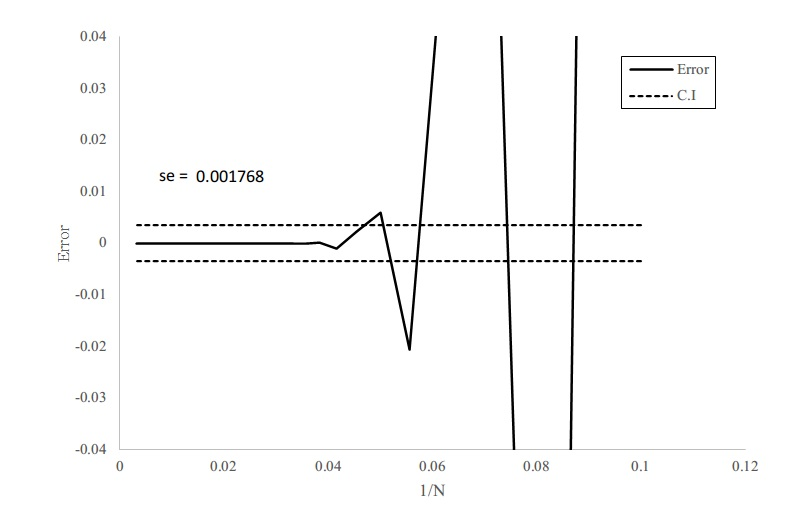
\includegraphics[width=0.8\linewidth]{value-plot-GBM-call.jpg}
    \caption[\emph{GBM-Call: Value accuracy comparing to the simulation with} $10^7$ \emph{paths.} ] {\emph{GBM-Call: Value accuracy comparing to the simulation with} $10^7$ \emph{paths.} \textbf{Note}: mean value from simulation = 6.885240, criteria of negligible error from the product of payoff function and density is $10^{-6}$, and $N$ starts from $10$ with increment $=2$.}

    \label{fig:label}
\end{figure}

\begin{figure}[H]
    \centering
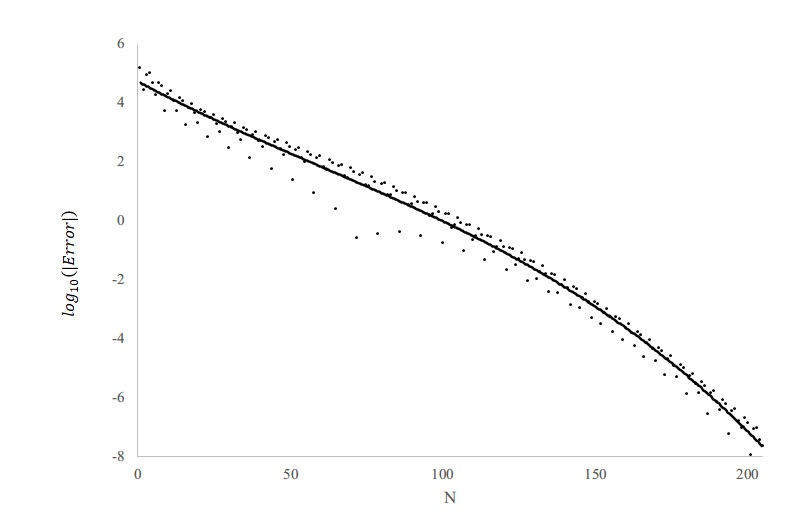
\includegraphics[width=0.8\linewidth]{error-plot-GBM-call.jpg}
    \caption[GBM-Call: \emph{The speed of error convergence.} ]{GBM-Call: \emph{The speed of error convergence.} \textbf{Note}: reference value $=6.8887285777$, criteria of negligible error from the product of payoff function and density is $10^{-15}$, $R^2=0.990$, and the regression line is $log_{10}\left(|Error|\right) = 0.0002N^2-0.0539N+4.7202$.}
    
    \label{fig:label}
\end{figure}

\subsection{Stochastic Volatility Model}
\begin{figure}[H]
    \centering
    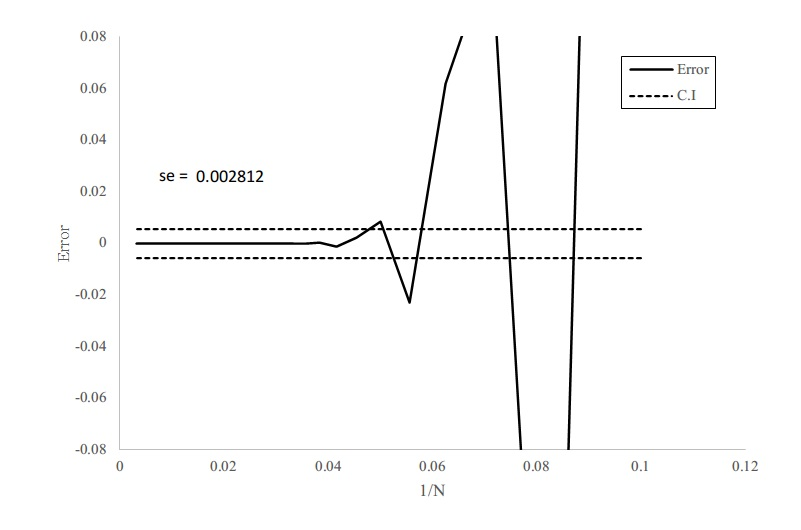
\includegraphics[width=0.8\linewidth]{value-plot-Heston-call.jpg}
    \caption[\emph{SV-Call: Value accuracy comparing to the simulation with} $10^7$ \emph{paths.}]{\emph{SV-Call: Value accuracy comparing to the simulation with} $10^7$ \emph{paths.} \textbf{Note}: mean value from simulation = 6.881753, criteria of negligible error from the product of payoff function and density is $10^{-6}$, and $N$ starts from $10$  with increment $=2$.}
    
    \label{fig:label}
\end{figure}

\begin{figure}[H]
    \centering
    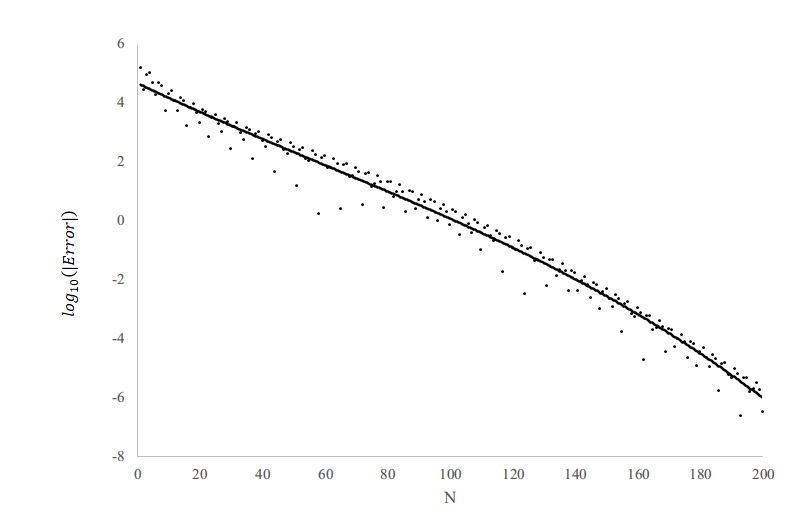
\includegraphics[width=0.8\linewidth]{error-plot-Heston-call.jpg}
    \caption[\emph{SV-Call: The speed of error convergence.}]{\emph{SV-Call: The speed of error convergence.} \textbf{Note}: reference value $=6.8816576853$, criteria of negligible error from the product of payoff function and density is $10^{-15}$, $R^2=0.989$, and the regression line is $log_{10}\left(|Error|\right) = 7.26\times 10^{-5}N^2-0.0482N+4.6371$.}
    \label{fig:label}
\end{figure}




\subsection{Log-normal Jump Diffusion Model}
\begin{figure}[H]
    \centering
    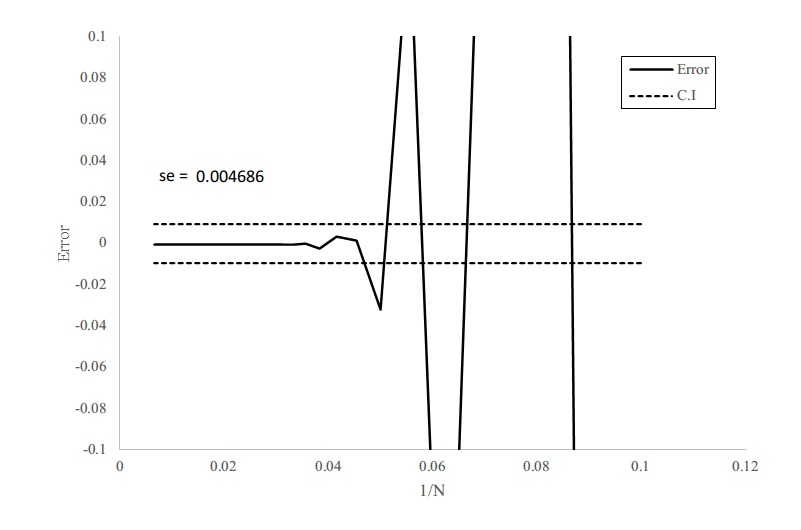
\includegraphics[width=0.8\linewidth]{value-plot-MJD-call.jpg}
    \caption[\emph{JD-Call: Value accuracy comparing to the simulation with}]{\emph{JD-Call: Value accuracy comparing to the simulation with} $10^7$ \emph{paths.} \textbf{Note}: mean value from simulation = 10.528850, criteria of negligible error from the product of payoff function and density is $10^{-6}$, and $N$ starts from $10$  with increment $=2$.}
    
    \label{fig:label}
\end{figure}

\begin{figure}[H]
    \centering
    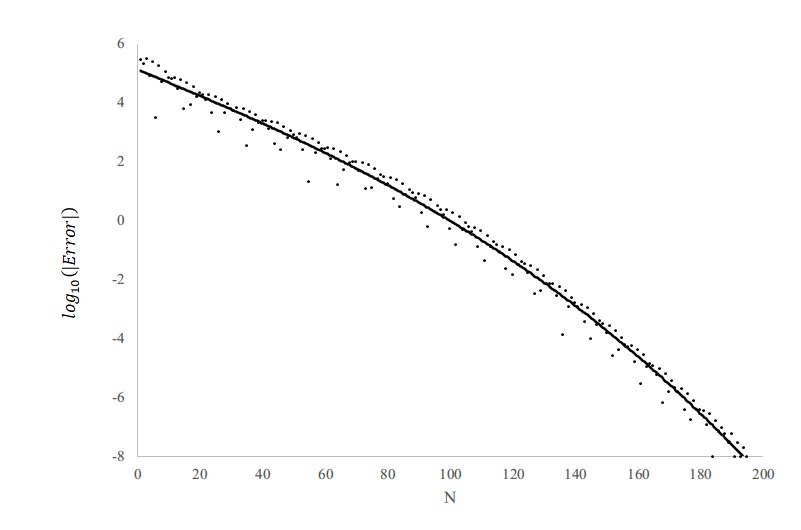
\includegraphics[width=0.8\linewidth]{error-plot-MJD-call.jpg}
    \caption[\emph{JD-Call: The speed of error convergence.}]{\emph{JD-Call: The speed of error convergence.} \textbf{Note}: reference value $=10.5281599666$, criteria of negligible error from the product of payoff function and density is $10^{-15}$, $R^2=0.994$, and the regression line is $log_{10}\left(|Error|\right) = -8.33\times 10^{-6}N^2-0.0448N+5.1472$.}

    \label{fig:label}
\end{figure}



\subsection{Double Exponential Jump Diffusion Model}
\begin{figure}[H]
    \centering
    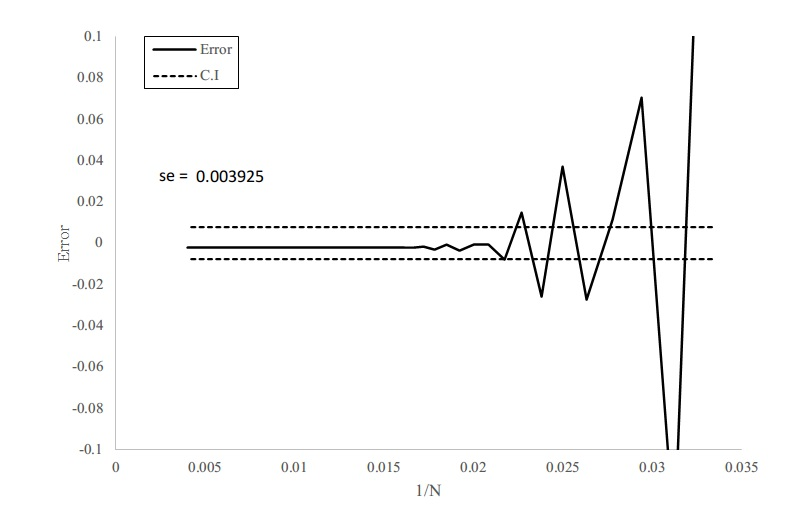
\includegraphics[width=0.8\linewidth]{value-plot-KJD-call.jpg}
    \caption[\emph{DJD-Call: Value accuracy comparing to the simulation with} $10^7$ \emph{paths.}]{\emph{DJD-Call: Value accuracy comparing to the simulation with} $10^7$ \emph{paths.} \textbf{Note}: mean value from simulation = 8.829095, criteria of negligible error from the product of payoff function and density is $10^{-6}$, and $N$ starts from $10$  with increment $=2$.}

    \label{fig:label}
\end{figure}

\begin{figure}[H]
    \centering
    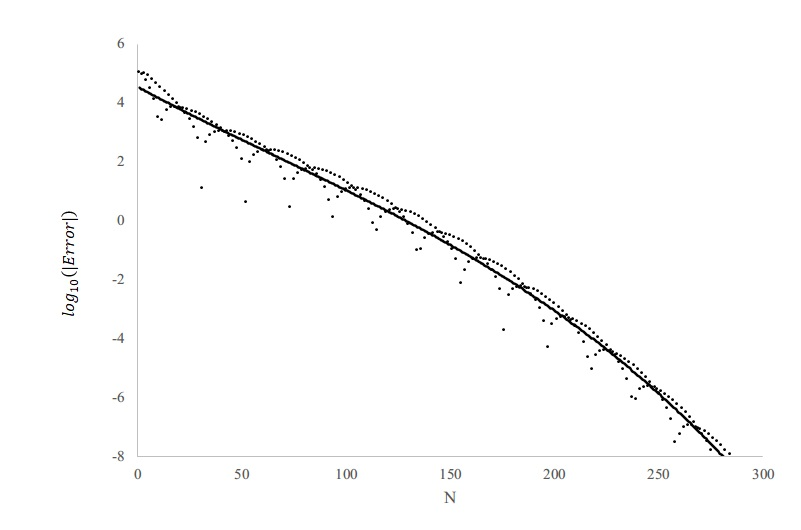
\includegraphics[width=0.8\linewidth]{error-plot-KJD-call.jpg}
    \caption[\emph{DJD-Call: The speed of error convergence.}]{\emph{DJD-Call: The speed of error convergence.} \textbf{Note}: reference value $=8.8270603863$, criteria of negligible error from the product of payoff function and density is $10^{-15}$, $R^2=0.990$, and the regression line is $log_{10}\left(|Error|\right) = -8.097\times 10^{-5}N^2-0.0402N+4.5899$.}
    
    \label{fig:label}
\end{figure}



\subsection{Stochastic Volatility Jump Model}
\begin{figure}[H]
    \centering
    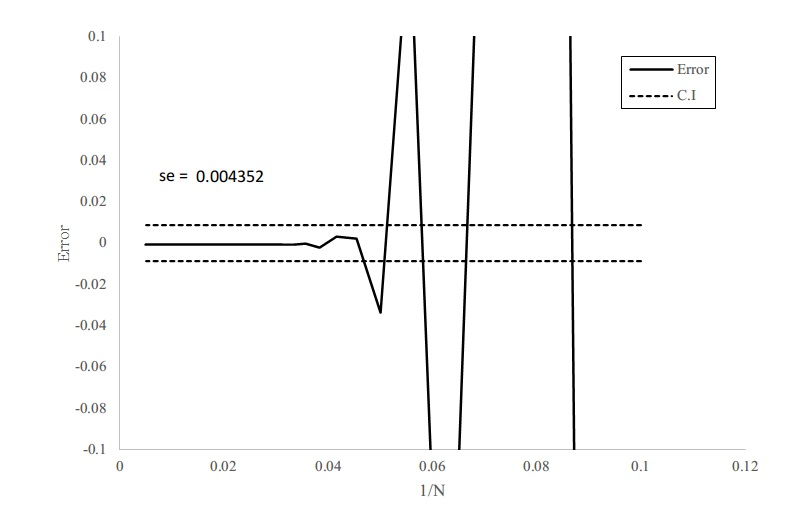
\includegraphics[width=0.8\linewidth]{value-plot-SVJ-call.jpg}
    \caption[\emph{SVJ-Call: Value accuracy comparing to the simulation with} $10^7$ \emph{paths.}]{\emph{SVJ-Call: Value accuracy comparing to the simulation with} $10^7$ \emph{paths.} \textbf{Note}: mean value from simulation = 10.525662, criteria of negligible error from the product of payoff function and density is $10^{-6}$, and $N$ starts from $10$  with increment $=2$.}
    
    \label{fig:label}
\end{figure}

\begin{figure}[H]
    \centering
    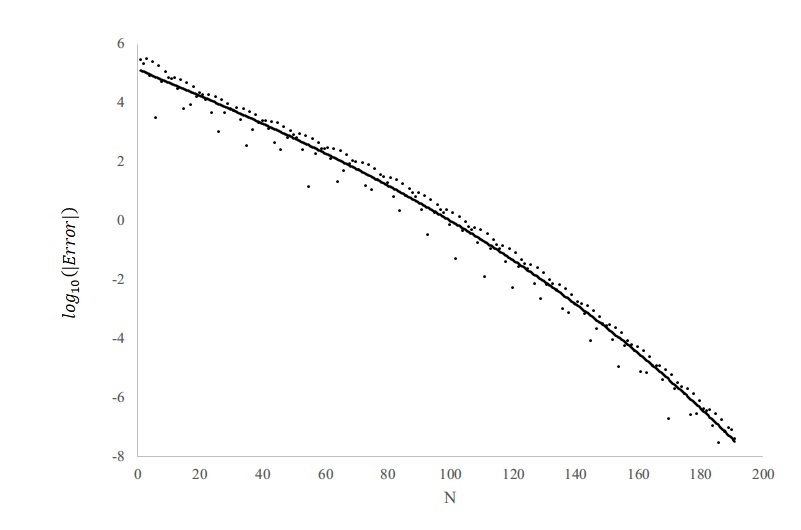
\includegraphics[width=0.8\linewidth]{error-plot-SVJ-call.jpg}
    \caption[\emph{SVJ-Call: The speed of error convergence.}]{\emph{SVJ-Call: The speed of error convergence.} \textbf{Note}: reference value $=10.5252142967$, criteria of negligible error from the product of payoff function and density is $10^{-15}$, $R^2=0.994$, and the regression line is $log_{10}\left(|Error|\right) = -2.395\times 10^{-5}N^2-0.0443N+5.1444$.}

    \label{fig:label}
\end{figure}



\subsection{Normal Inverse Gaussian Model}
\begin{figure}[H]
    \centering
    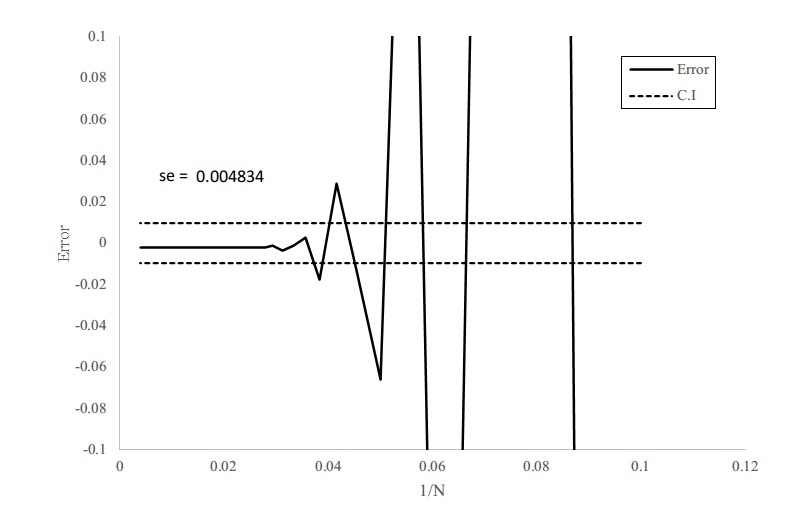
\includegraphics[width=0.8\linewidth]{value-plot-NIG-call.jpg}
     \caption[\emph{NIG-Call: Value accuracy comparing to the simulation with} $10^7$ \emph{paths.}]{\emph{NIG-Call: Value accuracy comparing to the simulation with} $10^7$ \emph{paths.} \textbf{Note}: mean value from simulation = 9.791681, criteria of negligible error from the product of payoff function and density is $10^{-6}$, and $N$ starts from $10$  with increment $=2$.}

    \label{fig:label}
\end{figure}
\begin{figure}[H]
    \centering
    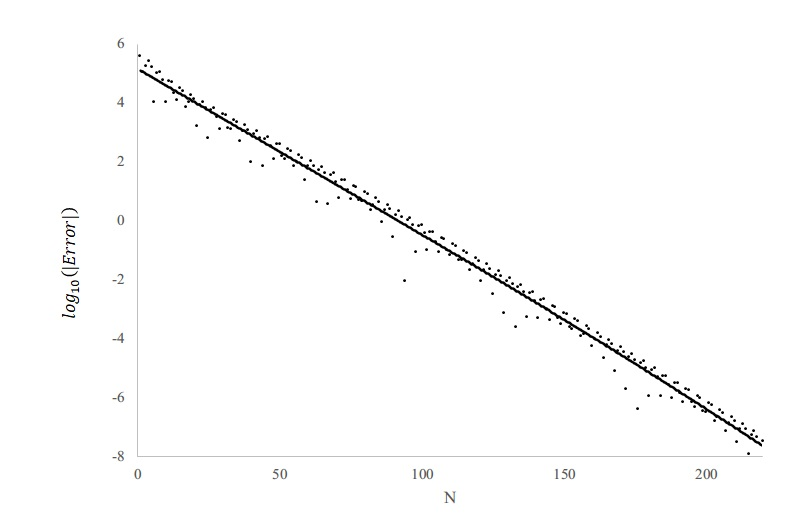
\includegraphics[width=0.8\linewidth]{error-plot-NIG-call.jpg}
    \caption[\emph{NIG-Call: The speed of error convergence.}]{\emph{NIG-Call: The speed of error convergence.} \textbf{Note}: reference value $=9.7896615158$, criteria of negligible error from the product of payoff function and density is $10^{-15}$, $R^2=0.991$, and the regression line is $log_{10}\left(|Error|\right) = 6.167\times 10^{-6}N^2-0.0562N+5.1576$.}
 
    \label{fig:label}
\end{figure}



\subsection{Variance Gamma Model}
\begin{figure}[H]
    \centering
    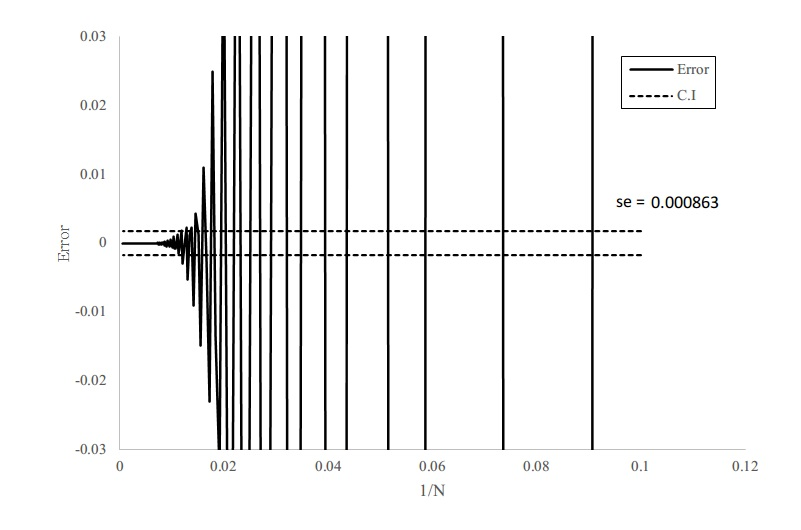
\includegraphics[width=0.8\linewidth]{value-plot-VG-call.jpg}
    \caption[\emph{VG-Call: Value accuracy comparing to the simulation with} $10^7$ \emph{paths.}]{\emph{VG-Call: Value accuracy comparing to the simulation with} $10^7$ \emph{paths.} \textbf{Note}: mean value from simulation = 6.885240, criteria of negligible error from the product of payoff function and density is $10^{-6}$, and $N$ starts from $10$  with increment $=2$.}
    
    \label{fig:label}
\end{figure}
\begin{figure}[H]
    \centering
    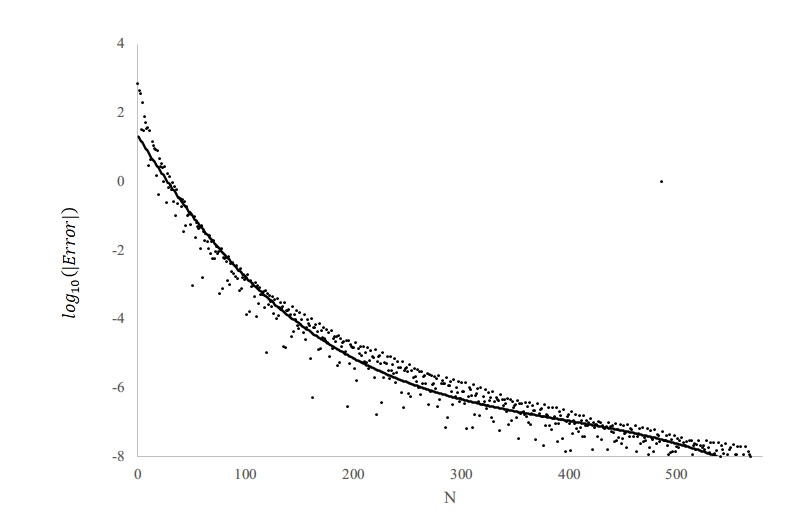
\includegraphics[width=0.8\linewidth]{error-plot-VG-call.jpg}
    \caption[\emph{VG-Call: The speed of error convergence.}]{\emph{VG-Call: The speed of error convergence.} \textbf{Note}: reference value $=6.8851648863$, criteria of negligible error from the product of payoff function and density is $10^{-15}$, $R^2=0.977$, and the regression line is $log_{10}\left(|Error|\right) = 0.0002N^2-0.07N+1.8948$.}

    \label{fig:label}
\end{figure}

\begin{figure}[ht]
    \begin{table}[H]
      \centering
      \caption[$log_{10}(|Error|)=AN^2+BN+C$]{Call - $log_{10}(|Error|)=AN^2+BN+C$}
    \end{table}
    
    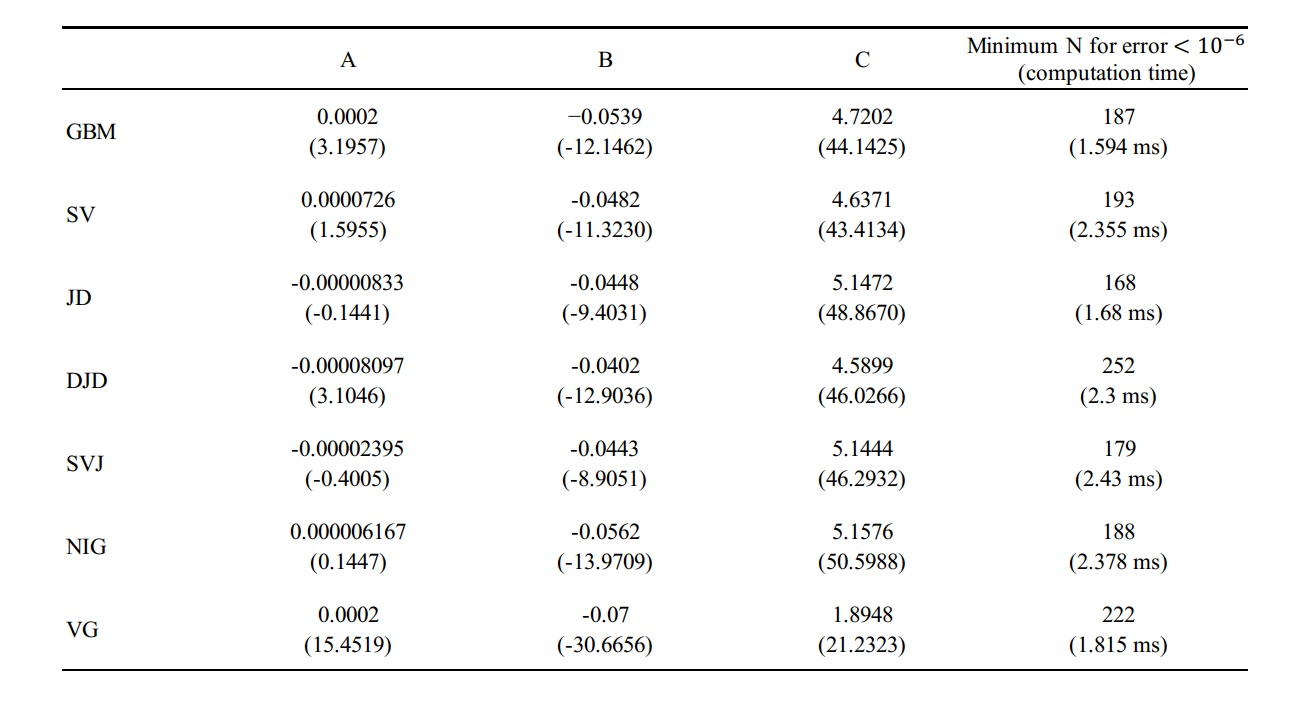
\includegraphics[width=1.1\textwidth,center]{call-table.jpg}
    \caption*{\small{This table reports the coefficients of the regression and t-statistics shown inside the parentheses in accordance with the coefficient. The time measurements in the final column are expressed in milliseconds and pertain to the MacBook Air equipped with the Apple M1 chip.}}
\end{figure}

% \begin{table}[ht]
% \caption[$log_{10}(|Error|)=AN^2+BN+C$]{Call - $log_{10}(|Error|)=AN^2+BN+C$}
% \centering
% \begin{tabular}{c c c }
%   \toprule
%   Coefficient 1 & Column 2 & Column 3 \\
%   \midrule
%   Value 1 & Value 2 & Value 3 \\
  
%   Value 4 & Value 5 & Value 6 \\
%   \bottomrule
% \end{tabular}
% \end{table}



I summarize the error convergence experimental results of the Call option in Table 3.1. The linear coefficients are all significantly negative, indicating that the model exhibits nearly exponential convergence. The quadratic coefficients, for the most part, are not significant, except for the geometric Brownian motion and the variance gamma model, but the coefficients are very small. Additionally, the computation time for all models is within 0.003 seconds, with an error on the order of $10^{-6}$. This demonstrates that the model is highly efficient for pricing call options.


\section{Convex Payoff for the Right End}
The one category of the payoff of the polynomial option is the convex payoff for the right end which has a payoff function where the leading coefficient is positive in $A \left(S_T\right)$. It means that the payoff function also tends to infinity as the stock price approaches infinity. As a polynomial option, the curve on the far right of the payoff function must be convex, meaning that the function has an infinite value on the right side. I call this category "Right Up".

To examine this polynomial option, the setting is $A(S_T)=0.05S_T^2-5S_T-20$. Then, the roots of $A(S_T)$ is $10\left( 5 - \sqrt{29} \right)$ and $10\left( 5 + \sqrt{29} \right)$. As a result, the positive interval that can be obtained $\left[0, \, 10\left( 5 - \sqrt{29} \right)\right]$, and $\left[ \, 10\left( 5 + \sqrt{29} \right),  \,\infty \right]$. All the following experiments are under $S_0=90$.

Note that the reference values for analyzing error convergence are calculated using binomial tree only for geometric Brownian motion. For other stochastic processes, these values are calculated under my model with $N=10^5$, because there are no analytical solution or tree-based methods for pricing polynomial options aside from geometric Brownian motion. These values fall within the confidence interval constructed by simulating $10^7$ paths within two standard errors. 

\newpage

\subsection{Geometric Brownian Motion}
\begin{figure}[H]
    \centering
    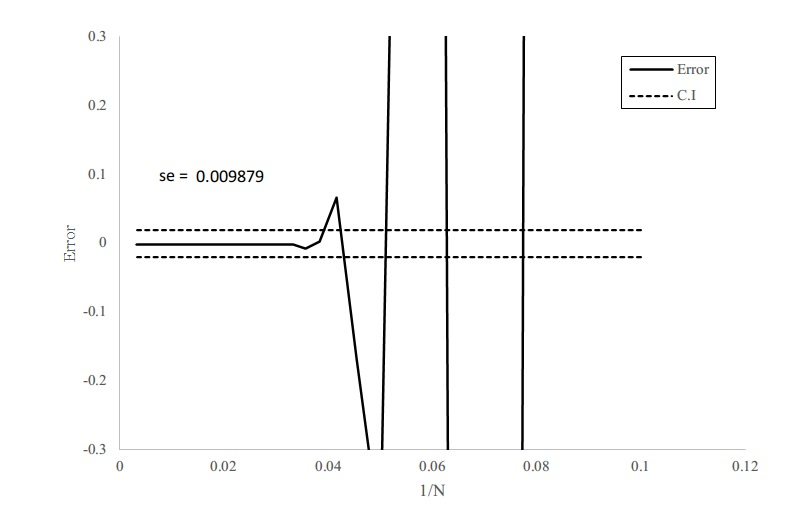
\includegraphics[width=0.8\linewidth]{value-plot-GBM-rightup.jpg}
    \caption[\emph{GBM-Up: Value accuracy comparing to the simulation with} $10^7$ \emph{paths.}]{\emph{GBM-Up: Value accuracy comparing to the simulation with} $10^7$ \emph{paths.} \textbf{Note}: mean value from simulation = 9.363655, criteria of negligible error from the product of payoff function and density is $10^{-6}$, and $N$ starts from $10$  with increment $=2$.}

    \label{fig:label}
\end{figure}

\begin{figure}[H]
    \centering
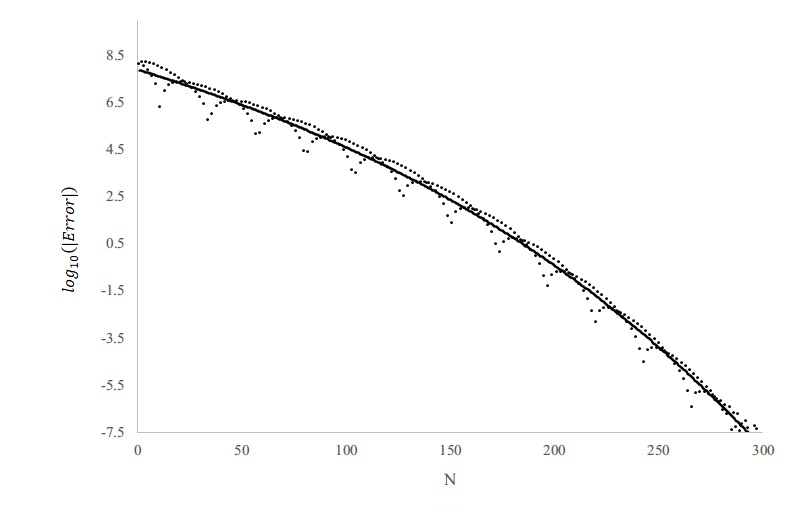
\includegraphics[width=0.8\linewidth]{error-plot-GBM-rightup.jpg}
    \caption[\emph{GBM-Up: The speed of error convergence.}]{\emph{GBM-Up: The speed of error convergence.} \textbf{Note}: reference value $=9.3619657891$, criteria of negligible error from the product of payoff function and density is $10^{-15}$, $R^2=0.995$, and the regression line is $log_{10}\left(|Error|\right) = -1.837\times 10^{-5}N^2-0.0295N+7.9392$.}

    \label{fig:label}
\end{figure}


\subsection{Stochastic Volatility Model}
\begin{figure}[H]
    \centering
    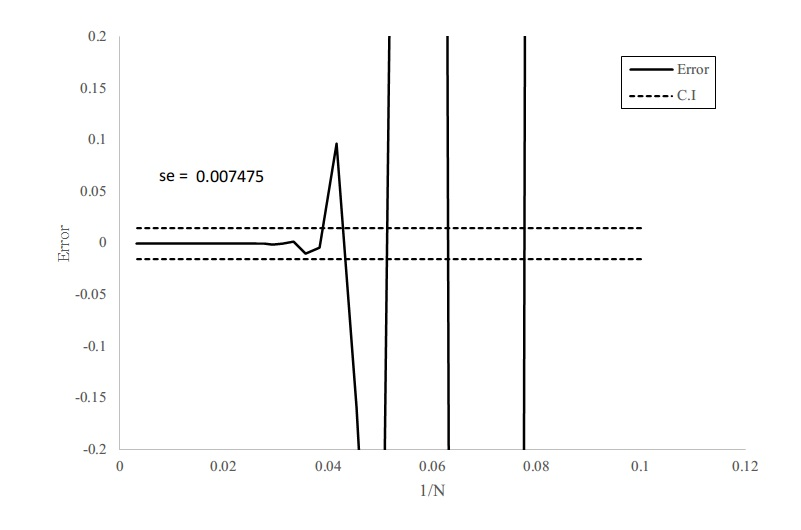
\includegraphics[width=0.8\linewidth]{value-plot-Heston-rightup.jpg}
    \caption[\emph{SV-Up: Value accuracy comparing to the simulation with} $10^7$ \emph{paths.}]{\emph{SV-Up: Value accuracy comparing to the simulation with} $10^7$ \emph{paths.} \textbf{Note}: mean value from simulation = 9.218680, criteria of negligible error from the product of payoff function and density is $10^{-6}$, and $N$ starts from $10$  with increment $=2$.}

    \label{fig:label}
\end{figure}
\begin{figure}[H]
    \centering
    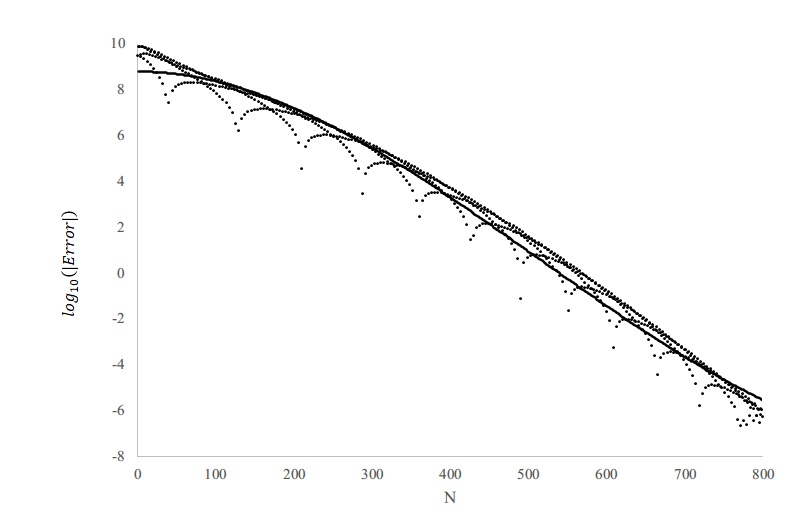
\includegraphics[width=0.8\linewidth]{error-plot-Heston-rightup.jpg}
    \caption[\emph{SV-Up: The speed of error convergence.}]{\emph{SV-Up: The speed of error convergence.} \textbf{Note}: reference value $=9.2180914622$, criteria of negligible error from the product of payoff function and density is $10^{-15}$, $R^2=0.994$, and the regression line is $log_{10}\left(|Error|\right) = -1.102\times 10^{-5}N^2-0.0107N+9.4685$.}
    
    \label{fig:label}
\end{figure}




\subsection{Log-normal Jump Diffusion Model}
\begin{figure}[H]
    \centering
    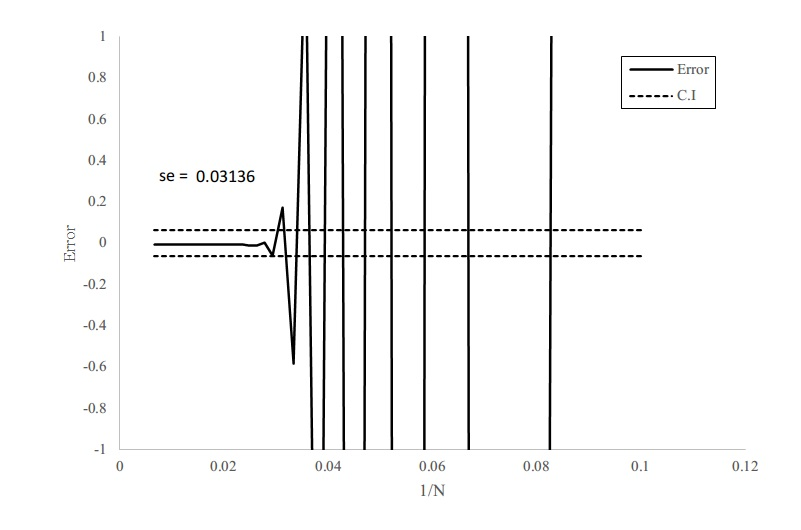
\includegraphics[width=0.8\linewidth]{value-plot-MJD-rightup.jpg}
    \caption[\emph{JD-Up: Value accuracy comparing to the simulation with} $10^7$ \emph{paths.}]{\emph{JD-Up: Value accuracy comparing to the simulation with} $10^7$ \emph{paths.} \textbf{Note}: mean value from simulation = 31.191878, criteria of negligible error from the product of payoff function and density is $10^{-6}$, and $N$ starts from $10$  with increment $=2$.}
    
    \label{fig:label}
\end{figure}

\begin{figure}[H]
    \centering
    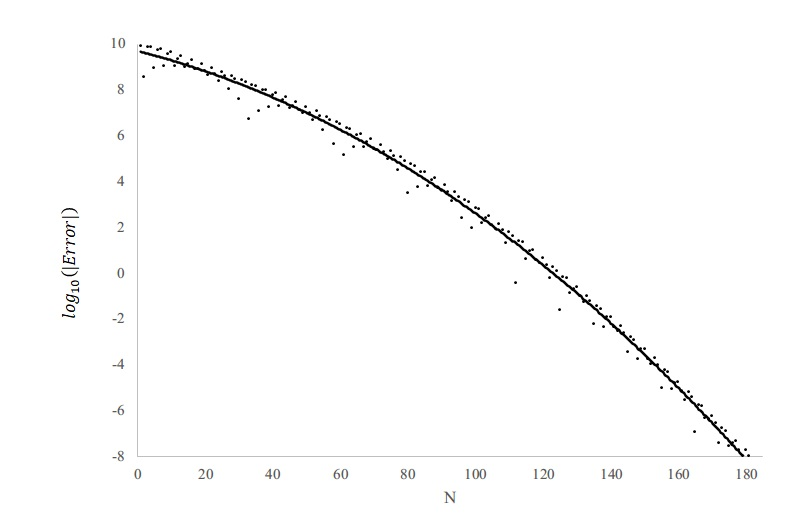
\includegraphics[width=0.8\linewidth]{error-plot-MJD-rightup.jpg}
    \caption[\emph{JD-Up: The speed of error convergence.}]{\emph{JD-Up: The speed of error convergence.} \textbf{Note}: reference value $=31.1831933197$, criteria of negligible error from the product of payoff function and density is $10^{-15}$, $R^2=0.996$, and the regression line is $log_{10}\left(|Error|\right) = -0.0003N^2-0.0367N+9.6889$.}

    \label{fig:label}
\end{figure}


\subsection{Double Exponential Jump Diffusion Model}
\begin{figure}[H]
    \centering
    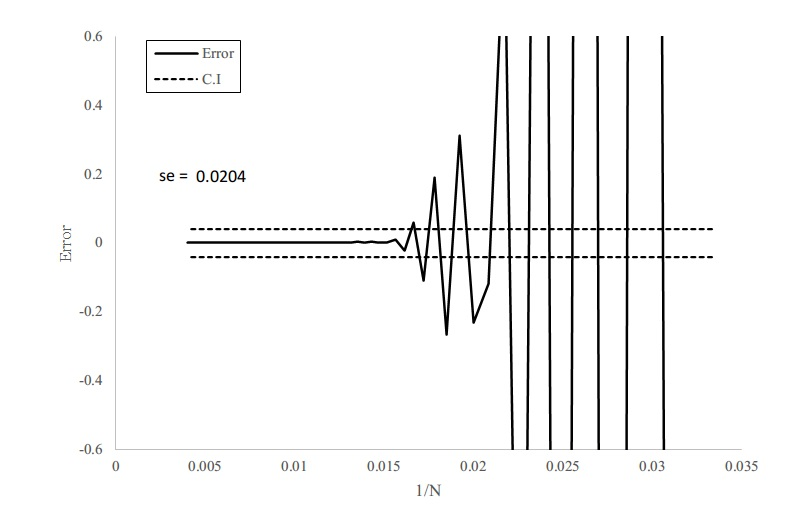
\includegraphics[width=0.8\linewidth]{value-plot-KJD-rightup.jpg}
     \caption[\emph{DJD-Up: Value accuracy comparing to the simulation with} $10^7$ \emph{paths.}]{\emph{DJD-Up: Value accuracy comparing to the simulation with} $10^7$ \emph{paths.} \textbf{Note}: mean value from simulation = 18.122275, criteria of negligible error from the product of payoff function and density is $10^{-6}$, and $N$ starts from $10$  with increment $=2$.}

    \label{fig:label}
\end{figure}

\begin{figure}[H]
    \centering
    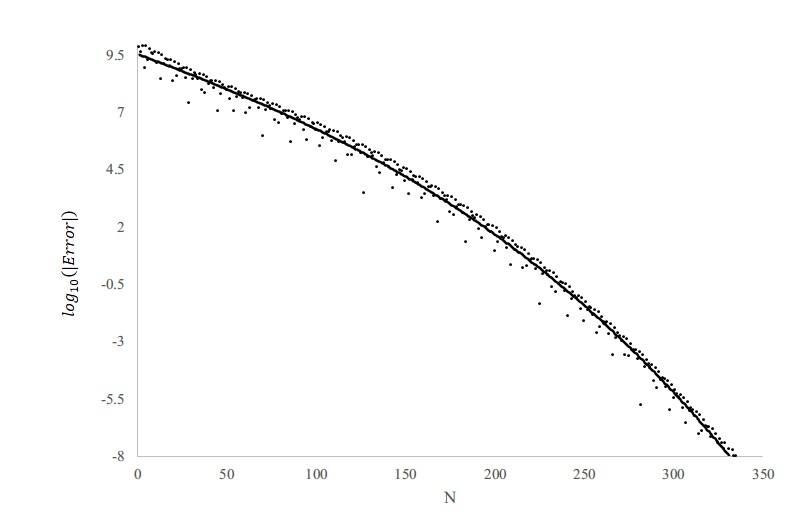
\includegraphics[width=0.8\linewidth]{error-plot-KJD-rightup.jpg}
    \caption[\emph{DJD-Up: The speed of error convergence.}]{\emph{DJD-Up: The speed of error convergence.} \textbf{Note}: reference value $=18.125462041$, criteria of negligible error from the product of payoff function and density is $10^{-15}$, $R^2=0.993$, and the regression line is $log_{10}\left(|Error|\right) = -8.375\times 10^{-6}N^2-0.0304N+9.9522$.}

    \label{fig:label}
\end{figure}


\subsection{Stochastic Volatility Jump Model}
\begin{figure}[H]
    \centering
    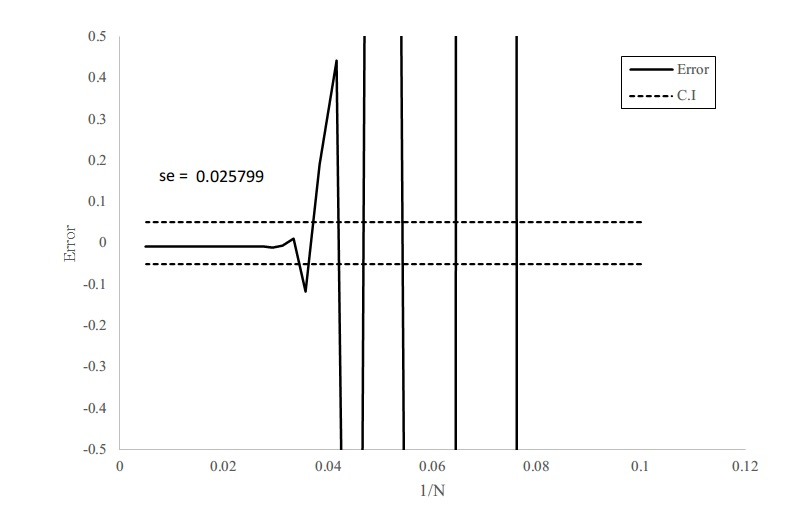
\includegraphics[width=0.8\linewidth]{value-plot-SVJ-rightup.jpg}
    \caption[\emph{SVJ-Up: Value accuracy comparing to the simulation with} $10^7$ \emph{paths.}]{\emph{SVJ-Up: Value accuracy comparing to the simulation with} $10^7$ \emph{paths.} \textbf{Note}: mean value from simulation = 31.12008, criteria of negligible error from the product of payoff function and density is $10^{-6}$, and $N$ starts from $10$  with increment $=2$.}

    \label{fig:label}
\end{figure}
\begin{figure}[H]
    \centering
    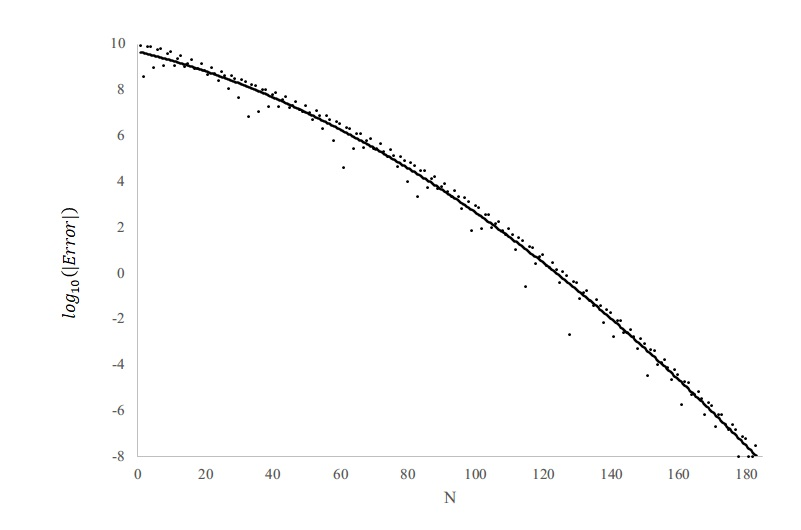
\includegraphics[width=0.8\linewidth]{error-plot-SVJ-rightup.jpg}
    \caption[\emph{SVJ-Up: The speed of error convergence.}]{\emph{SVJ-Up: The speed of error convergence.} \textbf{Note}: reference value $=31.1121085763$, criteria of negligible error from the product of payoff function and density is $10^{-15}$, $R^2=0.993$, and the regression line is $log_{10}\left(|Error|\right) = -0.0004N^2-0.0352N+9.6743$.}
    
    \label{fig:label}
\end{figure}


\subsection{Normal Inverse Gaussian Model}
\begin{figure}[H]
    \centering
    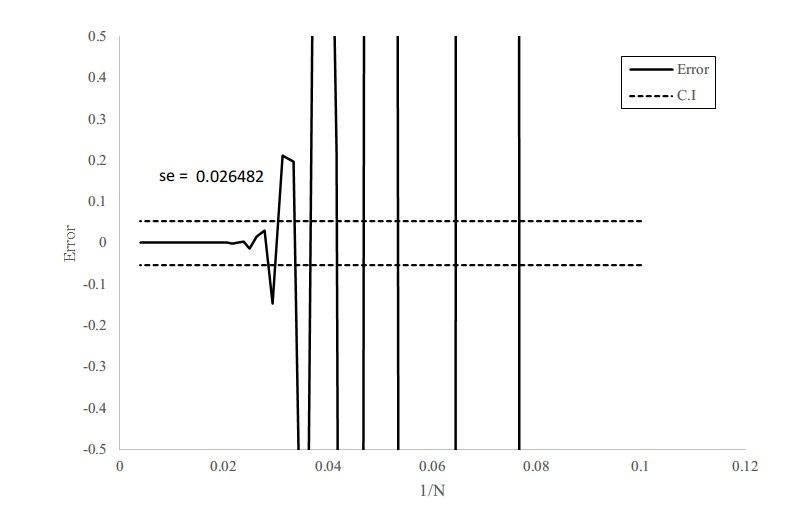
\includegraphics[width=0.8\linewidth]{value-plot-NIG-rightup.jpg}
    \caption[\emph{NIG-Up: Value accuracy comparing to the simulation with} $10^7$ \emph{paths.}]{\emph{NIG-Up: Value accuracy comparing to the simulation with} $10^7$ \emph{paths.} \textbf{Note}: mean value from simulation = 28.317193, criteria of negligible error from the product of payoff function and density is $10^{-6}$, and $N$ starts from $10$  with increment $=2$.}
 
    \label{fig:label}
\end{figure}

\begin{figure}[H]
    \centering
    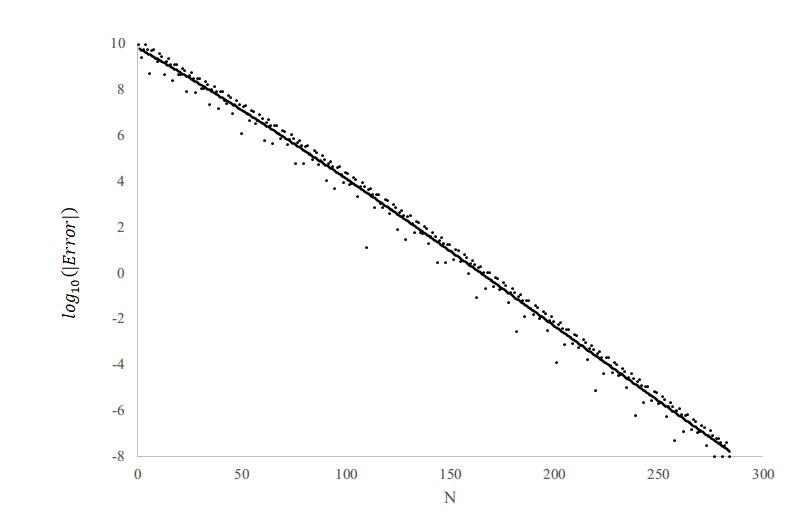
\includegraphics[width=0.8\linewidth]{error-plot-NIG-rightup.jpg}
    \caption[\emph{NIG-Up: The speed of error convergence.}]{\emph{NIG-Up: The speed of error convergence.} \textbf{Note}: reference value $=28.3185901456$, criteria of negligible error from the product of payoff function and density is $10^{-15}$, $R^2=0.991$, and the regression line is $log_{10}\left(|Error|\right) = -7.502\times 10^{-5}N^2-0.0508N+9.8393$.}

    \label{fig:label}
\end{figure}


\subsection{Variance Gamma Model}
\begin{figure}[H]
    \centering
    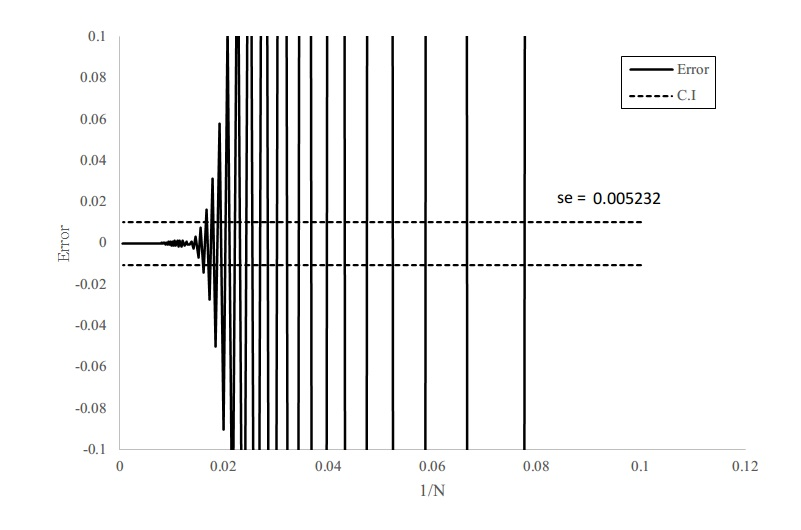
\includegraphics[width=0.8\linewidth]{value-plot-VG-rightup.jpg}
    \caption[\emph{VG-Up: Value accuracy comparing to the simulation with} $10^7$ \emph{paths.}]{\emph{VG-Up: Value accuracy comparing to the simulation with} $10^7$ \emph{paths.} \textbf{Note}: mean value from simulation = 8.219291, criteria of negligible error from the product of payoff function and density is $10^{-6}$, and $N$ starts from $10$  with increment $=2$.}

    \label{fig:label}
\end{figure}

\begin{figure}[H]
    \centering
    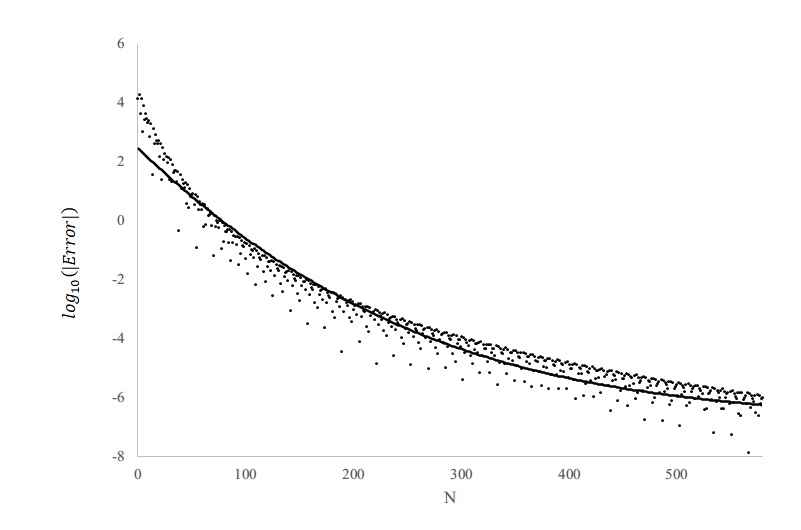
\includegraphics[width=0.8\linewidth]{error-plot-VG-rightup.jpg}
    \caption[\emph{VG-Up: The speed of error convergence.}]{\emph{VG-Up: The speed of error convergence.} \textbf{Note}: reference value $=8.219228342$, criteria of negligible error from the product of payoff function and density is $10^{-15}$, $R^2=0.972$, and the regression line is $log_{10}\left(|Error|\right) = 0.0001N^2-0.0535N+3.3449$.}

    \label{fig:label}
\end{figure}

\begin{figure}[ht]
    \begin{table}[H]
      \centering
      \caption[$log_{10}(|Error|)=AN^2+BN+C$]{Right Up - $log_{10}(|Error|)=AN^2+BN+C$}
    \end{table}
    \centering
        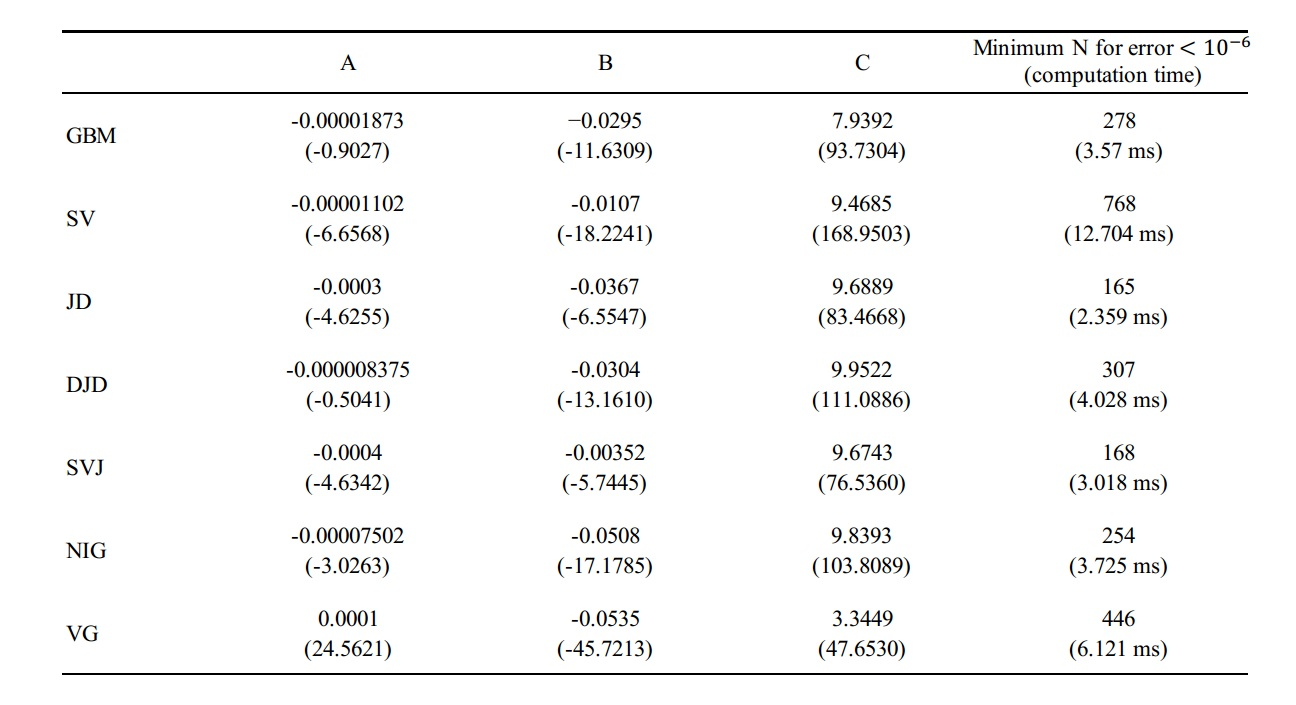
\includegraphics[width=1.1\textwidth,center]{rightup-table.jpg}
    \caption*{\small{This table reports the coefficients of the regression and t-statistics shown inside the parentheses in accordance with the coefficient. The time measurements in the final column are expressed in milliseconds and pertain to the MacBook Air equipped with the Apple M1 chip.}}
\end{figure}

Table 3.2 shows results that are very similar to those in Table 3.1. However, compared to the call option, the linear term becomes smaller and the quadratic term becomes more significant. This is because the payoff function grows faster compared to the call option, requiring a larger $N$ to achieve error convergence. Therefore, the significant negative coefficient of the quadratic term indicates slower error convergence initially, followed by faster error convergence. It can be observed that achieving an error below $10^{-6}$ requires a larger $N$. Additionally, the value of quadratic terms are still small. Although $N$ has increased, the computation time has not significantly increased, indicating that this model maintains a linear time complexity. Additionally, even for the stochastic volatility model with the highest $N$, it only requires 0.012 milliseconds to complete the calculation.



\section{Concave Payoff for the Right End}
In the other category of polynomial options, we discuss the payoff function of a polynomial option where the leading coefficient is negative. Because the polynomial has a negative leading coefficient, the curve on the far right side must be concave. For this payoff function, as the stock price approaches infinity, the payoff will always be zero. I call this category "Right Down".
To examine this polynomial option, the setting is $A(S_T)=-0.0031S_T^4+0.2358S_T^3-5.4793S_T^2+39.474S_T-44.235$ which is a high order polynomial function and with randomly chosen coefficients. Then, the roots of $A(S_T)$ is $1.363962$, $10.620047$, $25.599102$ and $38.481405$. As a result, the array of the positive intervals that can be obtained with $\left[0, \, 1.363962,\right]$, $ \left[10.620047, \, 25.599102\right]$, $\left[ 38.481405, \,\infty \right]$. All the following experiments are under $S_0=30$.

Note that the reference values for analyzing error convergence are calculated using binomial tree only for geometric Brownian motion. For other stochastic processes, these values are calculated under this model with $N=10^5$, because there are no analytical solutions or tree-based methods for pricing polynomial options aside from geometric Brownian motion. These values fall within the confidence interval constructed by simulating $10^7$ paths within two standard errors. 
\newpage

\subsection{Geometric Brownian Motion}
\begin{figure}[H]
    \centering
    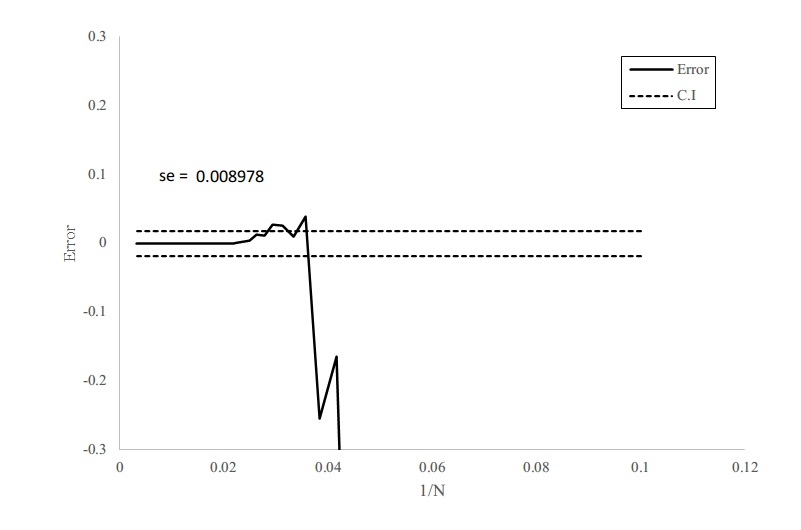
\includegraphics[width=0.8\linewidth]{value-plot-GBM-bothdown.jpg}
    \caption[\emph{GBM-Down: Value accuracy comparing to the simulation with} $10^7$ \emph{paths.}]{\emph{GBM-Down: Value accuracy comparing to the simulation with} $10^7$ \emph{paths.} \textbf{Note}: mean value from simulation = 48.755816, criteria of negligible error from the product of payoff function and density is $10^{-6}$, and $N$ starts from $10$  with increment $=2$.}
  
    \label{fig:label}
\end{figure}

\begin{figure}[H]
    \centering
    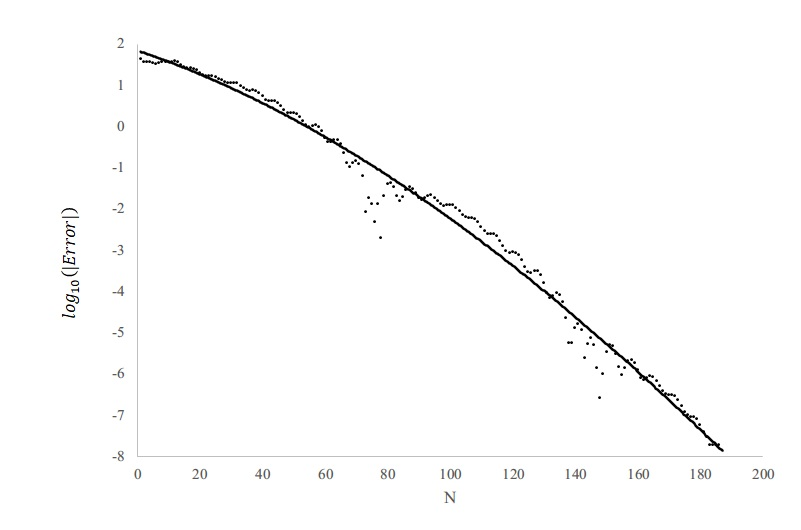
\includegraphics[width=0.8\linewidth]{error-plot-GBM-bothdown.jpg}
    \caption[\emph{GBM-Down: The speed of error convergence.}]{\emph{GBM-Down: The speed of error convergence.} \textbf{Note}: reference value $=48.7553402894$, criteria of negligible error from the product of payoff function and density is $10^{-15}$, $R^2=0.992$, and the regression line is $log_{10}\left(|Error|\right) = -0.0002N^2-0.0251N+1.8391$.}

    \label{fig:label}
\end{figure}


\subsection{Stochastic Volatility Model}
\begin{figure}[H]
    \centering
    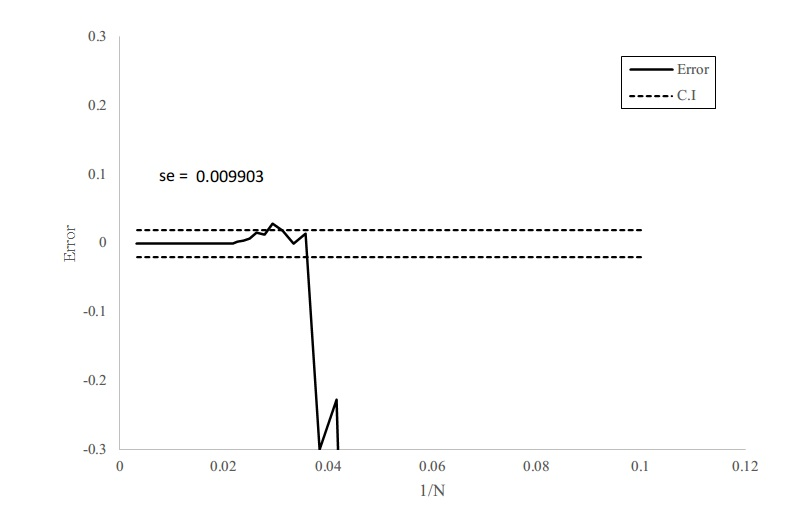
\includegraphics[width=0.8\linewidth]{value-plot-Heston-bothdown.jpg}
    \caption[\emph{SV-Down: Value accuracy comparing to the simulation with} $10^7$ \emph{paths.}]{\emph{SV-Down: Value accuracy comparing to the simulation with} $10^7$ \emph{paths.} \textbf{Note}: mean value from simulation = 49.003536, criteria of negligible error from the product of payoff function and density is $10^{-6}$, and $N$ starts from $10$  with increment $=2$.}

    \label{fig:label}
\end{figure}
\begin{figure}[H]
    \centering
    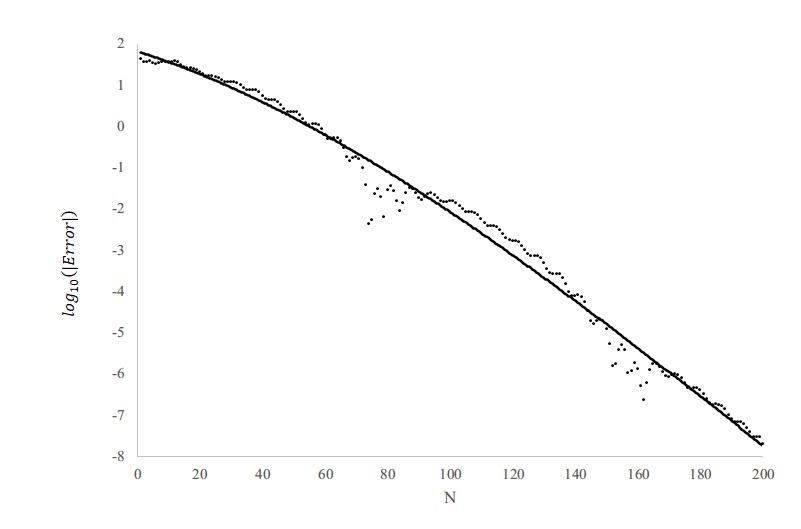
\includegraphics[width=0.8\linewidth]{error-plot-Heston-bothdown.jpg}
    \caption[\emph{SV-Down: The speed of error convergence.}]{\emph{SV-Down: The speed of error convergence.} \textbf{Note}: reference value $=49.0026564304$, criteria of negligible error from the product of payoff function and density is $10^{-15}$, $R^2=0.988$, and the regression line is $log_{10}\left(|Error|\right) = -0.0002N^2-0.0241N+1.8224$.}

    \label{fig:label}
\end{figure}


\subsection{Log-normal Jump Diffusion Model}
\begin{figure}[H]
    \centering
    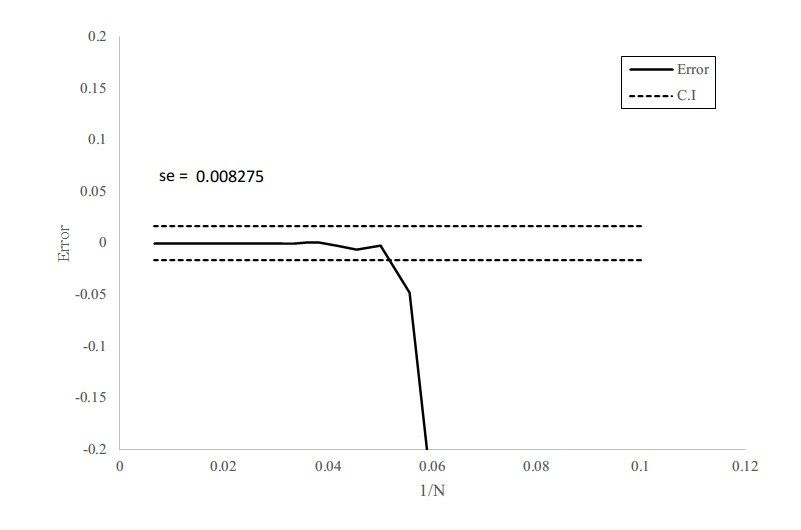
\includegraphics[width=0.8\linewidth]{value-plot-MJD-bothdown.jpg}
    \caption[\emph{JD-Down: Value accuracy comparing to the simulation with} $10^7$ \emph{paths.}]{\emph{JD-Down: Value accuracy comparing to the simulation with} $10^7$ \emph{paths.} \textbf{Note}: mean value from simulation = 33.154370, criteria of negligible error from the product of payoff function and density is $10^{-6}$, and $N$ starts from $10$  with increment $=2$.}

    \label{fig:label}
\end{figure}

\begin{figure}[H]
    \centering
    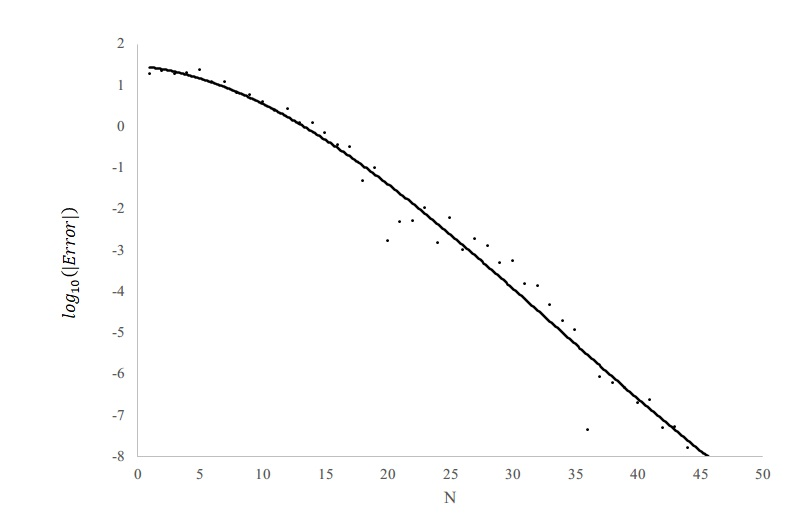
\includegraphics[width=0.8\linewidth]{error-plot-MJD-bothdown.jpg}
    \caption[\emph{JD-Down: The speed of error convergence.}]{\emph{DJD-Down: The speed of error convergence.} \textbf{Note}: reference value $=33.153704436$, criteria of negligible error from the product of payoff function and density is $10^{-15}$, $R^2=0.964$, and the regression line is $log_{10}\left(|Error|\right) = -0.0052N^2-0.0604N+1.5897$.}

    \label{fig:label}
\end{figure}


\subsection{Double Exponential Jump Diffusion Model}
\begin{figure}[H]
    \centering
    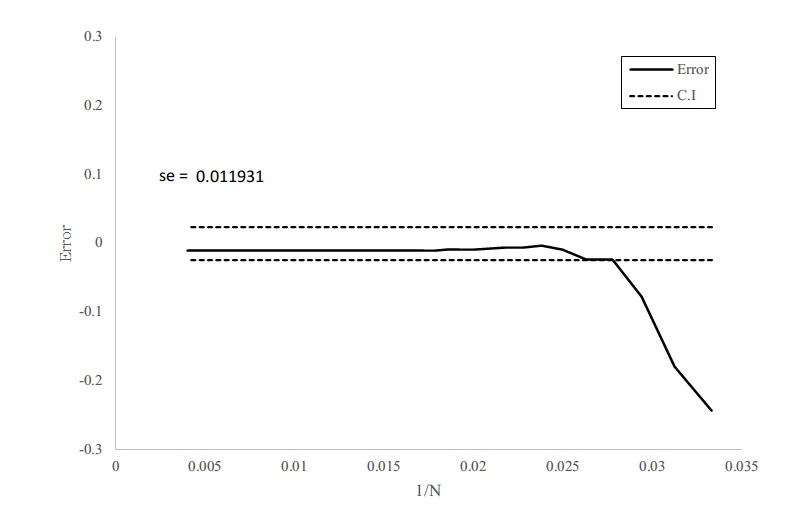
\includegraphics[width=0.8\linewidth]{value-plot-KJD-bothdown.jpg}
    \caption[\emph{DJD-Down: Value accuracy comparing to the simulation with} $10^7$ \emph{paths.}]{\emph{DJD-Down: Value accuracy comparing to the simulation with} $10^7$ \emph{paths.} \textbf{Note}: mean value from simulation = 43.817423, criteria of negligible error from the product of payoff function and density is $10^{-6}$, and $N$ starts from $10$  with increment $=2$.}

    \label{fig:label}
\end{figure}
\begin{figure}[H]
    \centering
    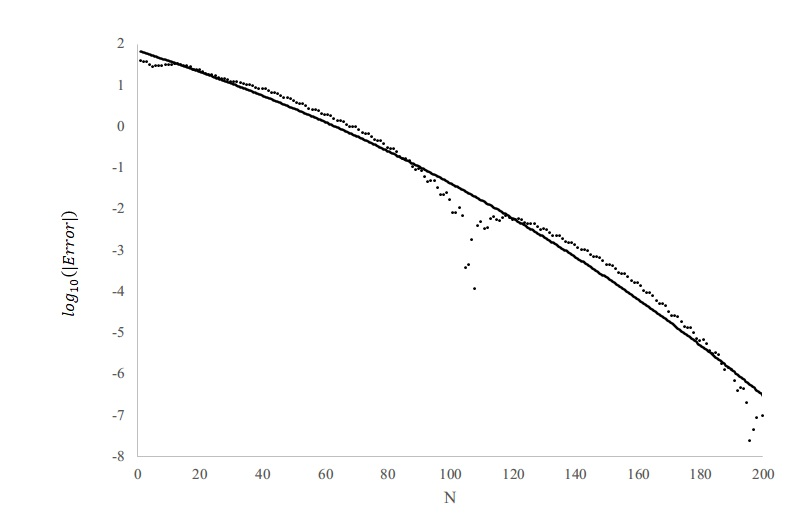
\includegraphics[width=0.8\linewidth]{error-plot-KJD-bothdown.jpg}
    \caption[\emph{DJD-Down: The speed of error convergence.}]{\emph{DJD-Down: The speed of error convergence.} \textbf{Note}: reference value $=43.8068018661$, criteria of negligible error from the product of payoff function and density is $10^{-15}$, $R^2=0.985$, and the regression line is $log_{10}\left(|Error|\right) = 1.039\times 10^{-5}N^2-0.0304N+1.9335$.}

    \label{fig:label}
\end{figure}



\subsection{Stochastic Volatility Jump Model}
\begin{figure}[H]
    \centering
    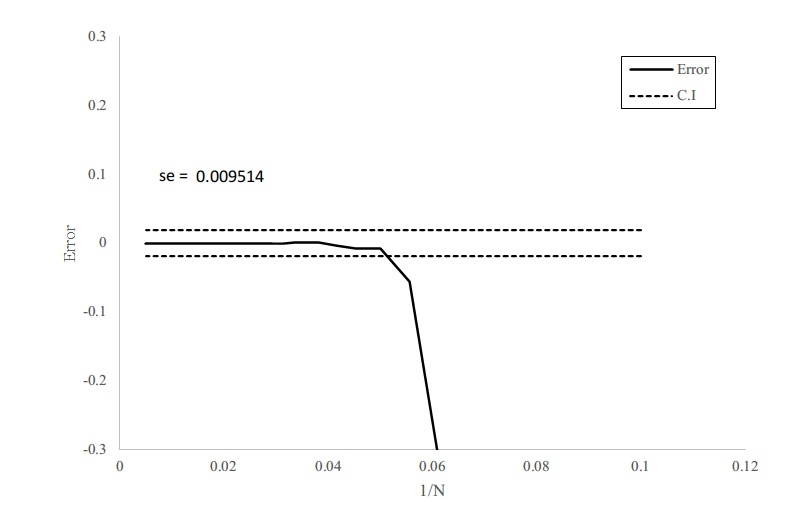
\includegraphics[width=0.8\linewidth]{value-plot-SVJ-bothdown.jpg}
    \caption[\emph{SVJ-Down: Value accuracy comparing to the simulation with} $10^7$ \emph{paths.}]{\emph{SVJ-Down: Value accuracy comparing to the simulation with} $10^7$ \emph{paths.} \textbf{Note}: the mean value from simulation = 33.197307, criteria of negligible error from the product of payoff function and density is $10^{-6}$, and $N$ starts from $10$  with increment $=2$.}

    \label{fig:label}
\end{figure}

\begin{figure}[H]
    \centering
    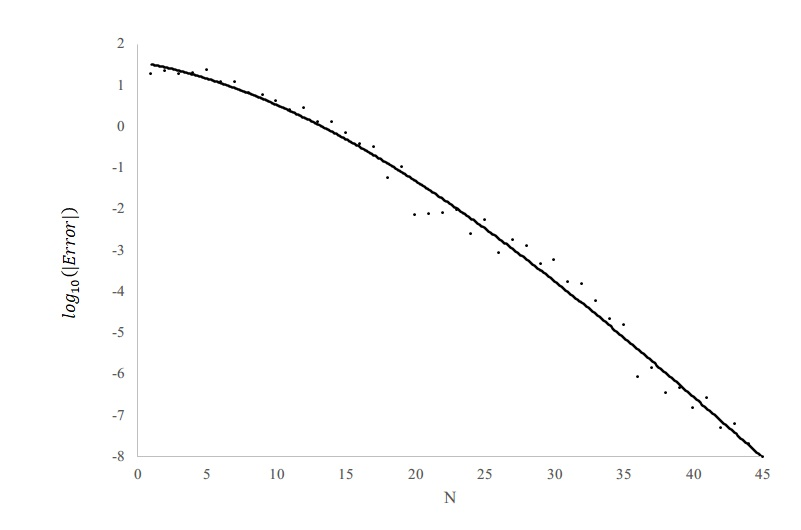
\includegraphics[width=0.8\linewidth]{error-plot-SVJ-bothdown.jpg}
    \caption[\emph{SVJ-Down: The speed of error convergence.}]{\emph{SVJ-Down: The speed of error convergence.} \textbf{Note}: reference value $=33.1970889218$, criteria of negligible error from the product of payoff function and density is $10^{-15}$, $R^2=0.985$, and the regression line is $log_{10}\left(|Error|\right) = -0.0052N^2-0.0058N+1.5678$.}

    \label{fig:label}
\end{figure}



\subsection{Normal Inverse Gaussian Model}
\begin{figure}[H]
    \centering
    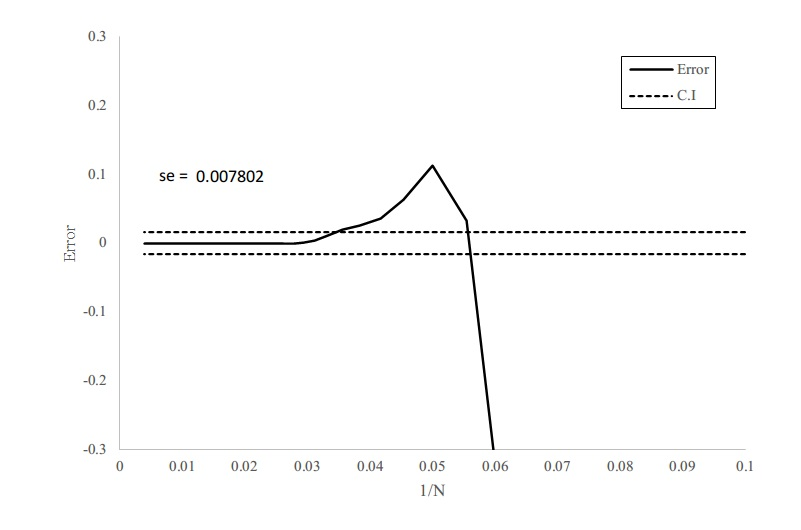
\includegraphics[width=0.8\linewidth]{value-plot-NIG-bothdown.jpg}
    \caption[\emph{NIG-Down: Value accuracy comparing to the simulation with} $10^7$ \emph{paths.}]{\emph{NIG-Down: Value accuracy comparing to the simulation with} $10^7$ \emph{paths.} \textbf{Note}: mean value from simulation = 35.340117, criteria of negligible error from the product of payoff function and density is $10^{-6}$, and $N$ starts from $10$  with increment $=2$.}

    \label{fig:label}
\end{figure}

\begin{figure}[H]
    \centering
    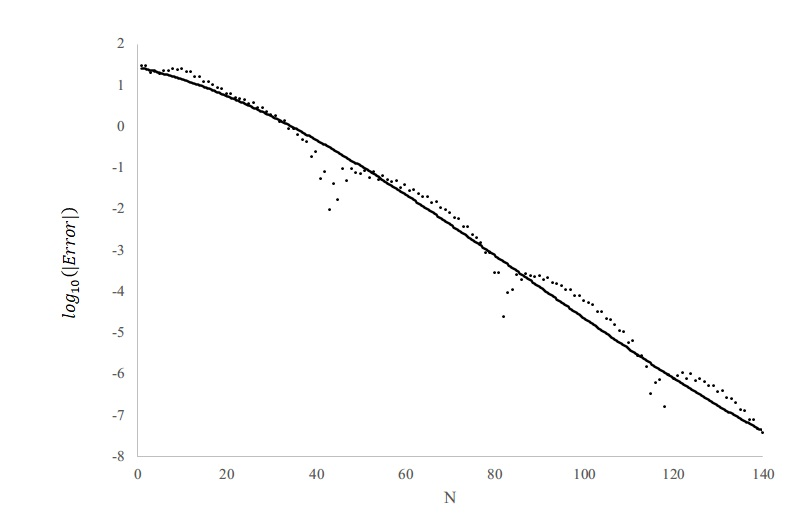
\includegraphics[width=0.8\linewidth]{error-plot-NIG-bothdown.jpg}
    \caption[\emph{NIG-Down: The speed of error convergence.}]{\emph{NIG-Down: The speed of error convergence.} \textbf{Note}: reference value $=35.3393903527$, criteria of negligible error from the product of payoff function and density is $10^{-15}$, $R^2=0.986$, and the regression line is $log_{10}\left(|Error|\right) = -0.0002N^2-0.0487N+1.7368$.}

    \label{fig:label}
\end{figure}


\subsection{Variance Gamma Model}
\begin{figure}[H]
    \centering
    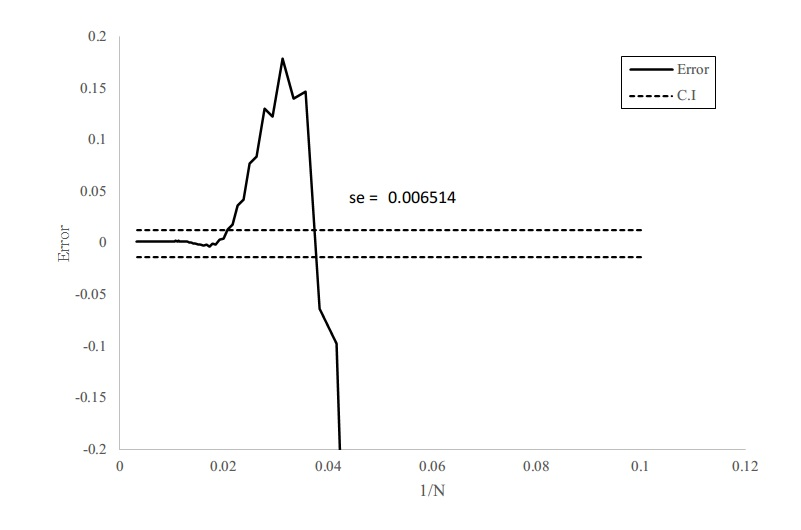
\includegraphics[width=0.8\linewidth]{value-plot-VG-bothdown.jpg}
    \caption[\emph{VG-Down: Value accuracy comparing to the simulation with} $10^7$ \emph{paths.}]{\emph{VG-Down: Value accuracy comparing to the simulation with} $10^7$ \emph{paths.} \textbf{Note}: mean value from simulation = 51.999204, criteria of negligible error from the product of payoff function and density is $10^{-6}$, and $N$ starts from $10$  with increment $=2$.}

    \label{fig:label}
\end{figure}

\begin{figure}[H]
    \centering
    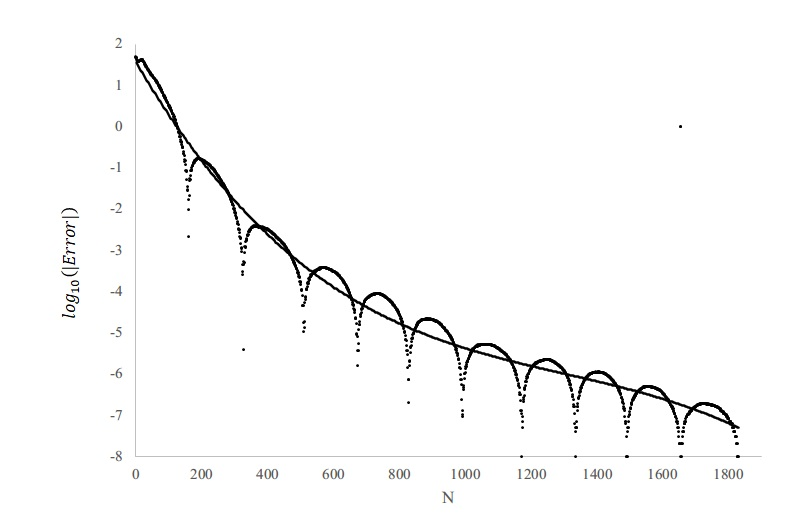
\includegraphics[width=0.8\linewidth]{error-plot-VG-bothdown.jpg}
    \caption[\emph{VG-Down: The speed of error convergence.}]{\emph{VG-Down: The speed of error convergence.} \textbf{Note}: reference value $=52.0009599216$, criteria of negligible error from the product of payoff function and density is $10^{-15}$, $R^2=0.972$, and the regression line is $log_{10}\left(|Error|\right) = 1.243\times 10^{-5}N^2-0.0173N+1.9176$.}

    \label{fig:label}
\end{figure}

\begin{figure}[ht]
    \begin{table}[H]
      \centering
      \caption[$log_{10}(|Error|)=AN^2+BN+C$]{Right Down - $log_{10}(|Error|)=AN^2+BN+C$}
    \end{table}
    \centering
        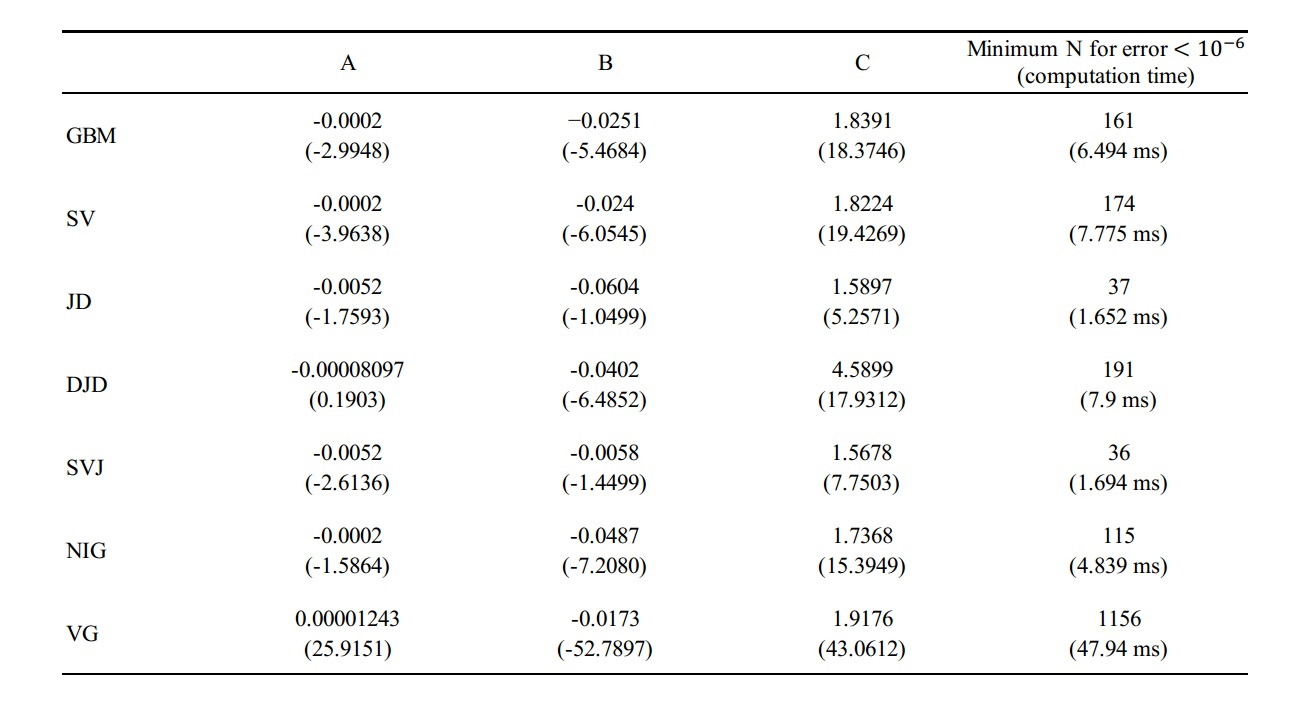
\includegraphics[width=1.1\textwidth,center]{bothdown-table.jpg}
    \caption*{\small{This table reports the coefficients of the regression and t-statistics shown inside the parentheses in accordance with the coefficient. The time measurements in the final column are expressed in milliseconds and pertain to the MacBook Air equipped with the Apple M1 chip.}}
\end{figure}

Under the concave payoff function for the right end, despite selecting a four-degree polynomial option, the highest degree term is larger than the call option and convex payoff for the right end in Table 3.2. However, compared to the convex payoff, it requires much fewer $N$. This is because, due to the property of the concave payoff function for the right end, the product of the payoff function and density function is zero on the far right. Therefore, there is no need to simulate over such a large range. As the interval between $l$ and $u$ increases, a larger $N$ is required for fitting. Furthermore, it also performs very well in terms of computation time, with a maximum time of only 0.0078 milliseconds to complete.


\section{Problem for Pricing Stochastic Double-Jump Stochastic Volatility Model}
The stochastic double jumps model is a widely recognized and valuable pricing model in the field of financial engineering. This stochastic process differs from other stochastic processes in that it incorporates jumps in both the variance and the rate of return simultaneously. However, during my attempts to apply this model for pricing purposes, we encountered an issue. Initially, I employed both simulation methods and numerical integration methods to price this stochastic process, and the results were consistent. However, when using my pricing approach, I discovered there is a division by zero error in computation. A singular point exists in the pricing process. To address this problem, let's provide a brief introduction to this stochastic process. Based on Duffie, Pan, and Singleton (2000) research, the process can be depicted by
\begin{align*}
d\left(\begin{array}{c}
Y_t \\
V_t
\end{array}\right)=\left(\begin{array}{c}
r-d-\lambda \mu-\frac{1}{2} V_t \\
\kappa_v\left(\bar{v}-V_t\right)
\end{array}\right) d t+\sqrt{V_t}\left(\begin{array}{cc}
1 & 0 \\
\bar{\rho} \sigma_v & \sqrt{1-\bar{\rho}^2} \sigma_v
\end{array}\right) d W_t^Q+d N_t,
\end{align*}
where $Y = \mathrm{ln}\left(S\right)$, $V$ is variance, $Z_t$ is a pure jump process in $\mathbb{R}^2$. The intensity of simultaneous correlated jumps in $Y$ and $V$ is $\lambda$. The distribution of the jump size in $V$ is exponential with mean $\mu_{c_v}$. The realization of jump size in $V$ is $z_v$. The jump size in $Y$ is a normal distribution with mean $mu_{c,y} + \rho_J z_v$ and variance $\sigma_{c,y}^2$. The characteristic function can be represented by
\begin{align*}
\varphi(v) & =\mathrm{exp}(\bar{\alpha} + \bar{\beta} \cdot V_0),
\end{align*}
where
\begin{align*}
\bar{\alpha} &= \alpha_0 + \lambda T \left(1 + \mu iv \right) + \lambda f, \\
\bar{\beta} &= -\frac{a\left(1 - \mathrm{e}^{-\gamma T}\right)}{2\gamma - \left(\gamma + b\right)\left(1 - \mathrm{e}^{-\gamma T}\right)},\\
\end{align*}
\begin{align*}
\alpha_0 &= -rT + \left(r - d\right)i v T, \\
&-k_v\bar{v}\left(\frac{\gamma + b}{\sigma_v^2}T +\frac{2}{\sigma_v^2}\mathrm{ln}\left[1-\frac{\gamma+b}{2\gamma}\left(1-\mathrm{e}^{-\gamma T}\right)\right]\right),\\
f &= \mathrm{exp}\left(\mu_{c,y} i v+\sigma_{c,y}^2\frac{v^2}{2}\right)\zeta, \\
a &= iv\left(1-iv\right),\\ 
b &= \sigma_v \bar{\rho} iv - k_v,\\
c &= 1 - \rho_J\mu_c^v u,\\ 
\gamma &= \sqrt{b^2 + a \sigma_v^2},\\ 
\mu &=\frac{\exp \left(\frac{1}{2} \sigma_{c, y}^2\right)}{1-\rho_J \mu_{c, v}},
\end{align*}
and
\begin{align}
\zeta &= \frac{\gamma-b}{(\gamma-b) c+\mu_{c, v} a} \tau \nonumber \\
&-\frac{2 \mu_{c, v} a}{(\gamma c)^2-\left(b c-\mu_{c, v} a\right)^2} \ln \left[1-\frac{(\gamma+b) c- \mu_{c, v} a}{2 \gamma c}\left(1-e^{-\gamma \tau}\right)\right]. \label{SVJJ problem}
\end{align}

When using this pricing formula, it is necessary to substitute $v=0$ into the characteristic function when calculating the first term of summation. However, this may cause problems. The denominator of the second part of $(\ref{SVJJ problem})$,
$$(\gamma c)^2-\left(b c-\mu_{c, v} a\right)^2 = 0,$$
where $\left(\gamma c\right)=bc$ and $\left(bc - \mu_{c,v}a\right)=bc$ because of $a=0$. It can be observed that this will result in the point being undefined in the complex space. Firstly, I attempted to replace $v=0$ with a very small number as a proxy for the limit in this method, but the results did not show significant changes. This value did not align with the results obtained from either the numerical integration method or the simulation method which deviates significantly from the confidence interval. In addition, I used the property of the characteristic function referencing Bakshi and Madan (2000), which says the value of the characteristic function equals 1 when $v=0$. However, this attempt did not alter the pricing results compared to using the first attempt of replacing with a limit proxy. I reviewed past research and found that, in most cases, the singularity position is replaced with a very small value or avoided by this point through numerical integration. Although some approaches are based on the Fourier method which is based on numerical integration, the methodologies are different from my method which is based on the Fourier expansion of density function. I believe that numerical integration methods are generally unaffected by the presence of singularities in the characteristic function, as long as these singular points are carefully avoided during the integration calculation. However, my method employed in the research necessitates a characteristic function free of singular points to accurately approximate the entire density function.\\

% !TeX root = ../main.tex
\chapter{Conclusions}
This study proposes a highly efficient pricing method for polynomial options, leveraging the Fourier method to exploit the relationship between the characteristic function and the coefficients in the Fourier-cosine expansion of the density function. The key advantage of this approach is its ability to separate the impact of the option payoff function and the underlying stochastic process, enabling it to accommodate a wide range of stochastic processes and payoff functions beyond plain vanilla options.

The research findings demonstrate that this pricing model exhibits a remarkably fast error convergence rate and excellent computational efficiency. Moreover, the study presents pricing results for various polynomial options, encompassing both convex and concave payoff functions for the right end. Notably, the proposed method accurately prices these complex polynomial options from first order to fourth order, with the error convergence rate remaining nearly exponential. Furthermore, to ensure the accuracy of pricing, we conducted a large number of Monte Carlo simulations within a highly stringent standard deviation, which corresponds to a very narrow confidence interval. Our pricing model consistently falls within the confidence interval, with the majority of results closely aligning with the mean value.

However, it encounters limitations when dealing with certain complex pricing models with singular points in their characteristic function, such as the stochastic double jumps model. To enhance the applicability of my pricing method and address the issue of singularities, future research could explore alternatives or develop more robust and flexible techniques for approximating the density function. Additionally, further investigation could be conducted to examine the impact of singularities on pricing accuracy and explore potential adjustments or modifications to improve the method's performance in such scenarios.


% 參考文獻
% References
\refmatter
\chapter*{Reference}
\begin{flushleft}
\hangindent=2em
\hangafter=1
[1] Bakshi and Madan. (2000), “Spanning and Derivative-Security Valuation,” \emph{Journal of Financial Economics}, 55, Vol. 2, 205–238.

\hangindent=2em
\hangafter=1
[2] Barndorff-Nielsen. (1997), “Processes of Normal Inverse Gaussian Type,” \emph{Finance and Stochastics}, 2, Vol. 1, 41–68.

\hangindent=2em
\hangafter=1
[3] Bates. (1996), “Jumps and Stochastic Volatility: Exchange Rate Processes Implicit in Deutsche Mark Options,” \emph{Review of Financial Studies}, 9, Vol. 1, 69–107. 

\hangindent=2em
\hangafter=1
[4] Carr and Madan. (1999), “Option Valuation Using the Fast Fourier Transform,” \emph{The Journal of Computational Finance}, 2, Vol. 4, 61–73.

\hangindent=2em
\hangafter=1
[5] Duffie, Pan, and Singleton. (2000), “Transform Analysis and Asset Pricing for Affine Jump-Diffusions,” \emph{Econometrica}, 68, Vol. 6, 1343–1376. 

\hangindent=2em
\hangafter=1
[6] Fang, and Oosterlee. (2009), “A Novel Pricing Method for European Options Based on Fourier-Cosine Series Expansions,” \emph{SIAM Journal on Scientific Computing }, 31, Vol. 2, 826–48.

\hangindent=2em
\hangafter=1
[7] Guo, Hung, and So. (2009), “A Generalization of the Barone-Adesi and Whaley Approach for the Analytic Approximation of American Options,” \emph{Journal of Futures Markets}, 29, Vol. 5, 478–493.

\hangindent=2em
\hangafter=1
[8] Heston. (1993), “A Closed-Form Solution for Options with Stochastic Volatility with Applications to Bond and Currency Options,” \emph{The Review of Financial Studies }, 6, Vol. 2, 327–343.

\hangindent=2em
\hangafter=1
[9] Kou. (2002), “A Jump-Diffusion Model for Option Pricing,” \emph{Management Science}, 48, Vol. 8, 1086-1101.

\hangindent=2em
\hangafter=1
[10] Lewis. (2001), “A Simple Option Formula for General Jump-Diffusion and Other Exponential Levy Processes,” \emph{SSRN Electronic Journal}. 

\hangindent=2em
\hangafter=1
[11] Macovschi and Quittard-Pinon. (2006), “On the Pricing of Power and Other Polynomial Options,” \emph{The Journal of Derivatives}, 13, Vol. 4, 61–71.

\hangindent=2em
\hangafter=1
[12] Madan, Carr, and Chang. (1998), “The Variance Gamma Process and Option Pricing,” \emph{Review of Finance}, 2, Vol. 1, 79–105.

\hangindent=2em
\hangafter=1
[13] Makate and Sattayatham. (2011), “Stochastic Volatility Jump-Diffusion Model for Option Pricing,” \emph{Journal of Mathematical Finance}, 1, Vol. 3, 90–97.

\hangindent=2em
\hangafter=1
[14] Merton. (1976), “Option Pricing When Underlying Stock Returns Are Discontinuous,” \emph{Journal of Financial Economics}, 3, Vol. 1–2, 125–144.

\hangindent=2em
\hangafter=1
[15] Wang J.Y., Wang C.J., Dai, Chen, Liu, and Zhou. (2022), “Efficient and Robust Combinatorial Option Pricing Algorithms on the Trinomial Lattice for Polynomial and Barrier Options,” \emph{Mathematical Problems in Engineering}, Vol. 2022.
\end{flushleft}

% % 附錄
% % Appendices
% % !TeX root = ../main.tex

\appendix{A}{模型參數表}
\section{模型一}
\section{模型二}

% % !TeX root = ../main.tex

\appendix{B}{BraTS 2021分割結果圖}
\section{編號 0001~0050}
\section{編號 0051~0100}


\end{document}
